\chapter{Ethnographie über das Handwerk des Fliesenlegers}

\section{Persönlicher Bezug}

Um meine Beobachtungen besser einordnen zu können, soll hier mein persönlicher Bezug zum Handwerk des Fliesenlegers und handwerklichen Berufen generell dargelegt werden. Ich absolvierte weder eine Ausbildung zum Fliesenleger, noch zu einem anderen handwerklichen Beruf. Meine Hobbies waren zwar bis jetzt immer im technischen Bereich angesiedelt, jedoch bezogen sie sich auf Computer und Smartphones, welche ich seit dem Start meines Studiums selbst repariere. Mit Maschinen, wie Autos oder Motorrädern beschäftigte ich mich hingegen weniger. 

Ich arbeitete nach dem Abitur als Aushilfe in einer Praktiker Filiale, wodurch ich sporadisch mit Baustoffen vertraut gemacht wurde. Diese Erfahrung half mir bei meinem Praktikum, da ich die Baustoffe kannte, mit denen wir täglich umgegangen sind und wusste wie man diese handhabt. Zusätzlich bin ich sportlich, was vorteilhaft für den körperlich anspruchsvollen Beruf eines Handwerkers ist, bei dem man oft schwer tragen muss.

In diesem Praktikum sammelte ich also meine ersten Erfahrungen in einem Handwerklichen Beruf. Ich traf den Fliesenleger bei einem Vorgespräch zum Praktikum, bei dem ich ihm meine Masterarbeit vorstellte, zum ersten Mal. Er leitet seit 25 Jahren einen Ein-Mann-Betrieb und ist in seiner Umgebung sehr bekannt und angesehen. In seiner Laufbahn erhielt er sporadisch Unterstützung durch Praktikanten oder andere Fliesenleger, arbeitete jedoch sonst allein. Er wusste also wie man mit Praktikanten umgeht und konnte mir so passend Wissen vermitteln.

\section{Ziel der Ethnographie}

Da ich nie als Fliesenleger arbeitete, sollte mir das Praktikum einen Einblick in das Handwerk geben, um Möglichkeiten zu finden, mit technischen Mitteln, die Arbeit zu erleichtern oder zu beschleunigen. Mein erstes Ziel war es, Ansatzpunkte zu finden, wo ein Fliesenleger Unterstützung brauchen kann. Also Arbeitsschritte zu identifizieren, die unnötig lang dauern, um erledigt zu werden oder umständlich sind.

Als Zweites suchte ich nach Möglichkeiten der Unterstützung, bei welchen speziell Augmented Reality nützlich sein kann. Wo also der Einsatz von AR einen Mehrwert für den Handwerker erzeugen kann.

Durch meine persönliche Mithilfe bei der Arbeit, erhielt ich einen tiefen Einblick in die Arbeit eines Fliesenlegers. Im nächsten Abschnitt erkläre ich, wie ich die erlebten Erfahrungen festgehalten habe.

\section{Durchführung der Ethnographie}

Bei meiner Beobachtung übernahm ich die Aufgabe des Praktikanten. Ich erledigte also kleinere Aufgaben, wie beispielsweise das Verfugen der Fliesen, und arbeitete dem Fliesenleger durch Tätigkeiten, wie das Tragen und Reichen der Fliesen zu. Der Fliesenleger übernahm das Legen der Fliesen selbst, weil er dies nach Augenmaß macht, dafür Erfahrung notwendig ist und dies die Qualität seiner Arbeit am meisten auszeichnet. Genauere Informationen dazu sind dem nächsten Kapitel „Ablauf und Ergebnisse der Ethnographie“ zu entnehmen.

Zur Dokumentation nutzte ich einen Notizblock, auf welchen ich meine Beobachtungen aufschrieb. Tonaufnahmen machte ich während des gesamten Praktikums keine, da diese Aufgrund der Baugeräusche unbrauchbar geworden wären und ihr Inhalt nicht viel beigetragen hätte. Ich hatte im Laufe des Tages zwischen Aufgaben Zeit oder nahm mir während kleineren Aufgaben Zeit, um Notizen zu machen. Da der Fliesenleger wusste, dass ich das Praktikum für meine Masterarbeit mache, war es kein Problem und auch für die Arbeit nicht hinderlich. Auch während der Arbeit stellte ich viele Fragen und schrieb mir die Antworten auf. Er erklärte alle Schritte, vor und während der Ausführung, damit ich die Zusammenhänge besser verstehe. Zusätzlich vervollständigte ich während den Pausen, als auch während Besorgungsfahrten in das Lager oder um Material zu kaufen, meine Notizen. Nach einem Arbeitstag bereitete ich die Informationen nach und fügte fehlende Informationen beziehungsweise Informationen, die mir erst im Nachhinein aufgefallen sind hinzu. Generell sprachen wir an den Tagen viel miteinander. Er erklärte viel von sich aus und ich stellte viele Fragen. So bekam ich ein umfangreiches Bild seiner Arbeit.

Insgesamt dauerte das Praktikum knapp zwei Wochen, vom 30.07.2018 bis zum 10.08.2018. Jeden Tag waren wir ca. von 8 Uhr bis 15 Uhr auf einer Baustelle.

Meine Aufzeichnungen fertigte ich in chronologischer Reihenfolge an. Für diese Arbeit und einen Leser ist das jedoch wenig sinnvoll die Informationen in dieser Reihenfolge aufzunehmen. Deswegen fasse ich in dieser Ethnographie die Arbeit der einzelnen Tage zusammen und gebe sie als Text, welcher den Ablauf des Fliesens eines Bades beschreibt, wieder. Die Ausführungen beginnen also beim Kundengespräch im Rohbau eines Raumes und enden in einem fertigen Badezimmer. Im Laufe meines Praktikums durchlief ich dazu alle Schritte, jedoch in unterschiedlicher Reihen-folge und auf vielen verschiedenen Baustellen. Zur Zeit des Beginns meines Praktikums bearbeitete der Fliesenleger nämlich mehrere offene Baustellen und nahm zeitgleich auch neue Projekte auf. Durch diese Anordnung der Ereignisse bekommt der Leser einen Gesamteindruck, wie die Arbeit eines Fliesenlegers aussieht und kann besser nachvollziehen wo und wie ich meine Ansätze für oben genannte Ziele fand.

\section{Ablauf und Ergebnisse der Ethnographie}

\subsection{Planung: Kundengespräch}

Ich fragte den Fliesenleger, bevor wir zur ersten Baustelle fuhren, wie Kundengespräche bei ihm normalerweise ablaufen. Dieser sagte mir, es gibt zwei Situationen:

\begin{itemize}
	\item Der Kunde hat bereits eine genaue Vorstellung, wie der Raum gefliest werden soll.
	\item Der Kunde hat keine genaue Vorstellung des Endergebnisses und verlässt sich auf die Beratung durch den Fliesenleger.
\end{itemize}

Bei ersterem hört er sich den Plan des Kunden an und bietet ihm zusätzlich beratend eigene Vorschläge an. Teilweise möchten Kunden das nicht und beharren darauf ihre Vorstellungen genau umgesetzt zu bekommen. Er persönlich führt solche Aufträge teilweise nicht durch. Dazu kommt es, wenn ein Kunde etwas umgesetzt haben möchte, was er für schlechte Praxis hält, da das die generelle Qualität seiner Arbeit schmälern und spätere Mängel auf ihn zurückfallen. 

In zweiterem Szenario legt der Fliesenleger dem Kunden seine Vorstellungen des fertigen Raumes dar. Dieser kann dann seine Meinung dazu äußern, Anregungen geben und Änderungen vorschlagen. Laut dem Fliesenleger können Kunden sich das Ergebnis aber im leeren Rohbau nicht vorstellen und überlassen ihm als Profi die komplette Planung. Eine persönliche Note im Bad zu hinterlassen und guten Kundenbezug aufzubauen sieht der Fliesenleger dabei als sein Markenzeichen.

Auf einer Baustelle arbeiten oft verschiedene Handwerker, wie Maurer, Trockenbauer, Installateur und Fliesenleger zusammen. Es ist von Vorteil, wenn sie zusammen planen, um von Anfang an festzulegen wo beispielsweise Dusche, Badewanne, Toilette und Waschbecken positioniert werden sollen. Für diese Elemente gibt es DIN Normen die eingehalten werden müssen. Eine Toilette muss zum Beispiel in einem gewissen Abstand über dem Boden aufgehängt werden. Wenn dieser Plan vorher festgelegt wird, vereinfacht das die Zusammenarbeit enorm. Auf der Baustelle auf der ich meine Beobachtungen machte, waren diese Planungen bereits abgeschlossen. Es ging also nur noch um das Vorbereiten und Verlegen der Fliesen.

Der Kunde, mit welchem wir das Kundengespräch führten war selbst Handwerker, Elektriker. Er hatte auf Baustellen schon mit Fliesenlegern zusammengearbeitet, wodurch er deren Planung und Arbeit besser einschätzen konnte. 

\begin{figure}[h]
	\begin{center}
		\noindent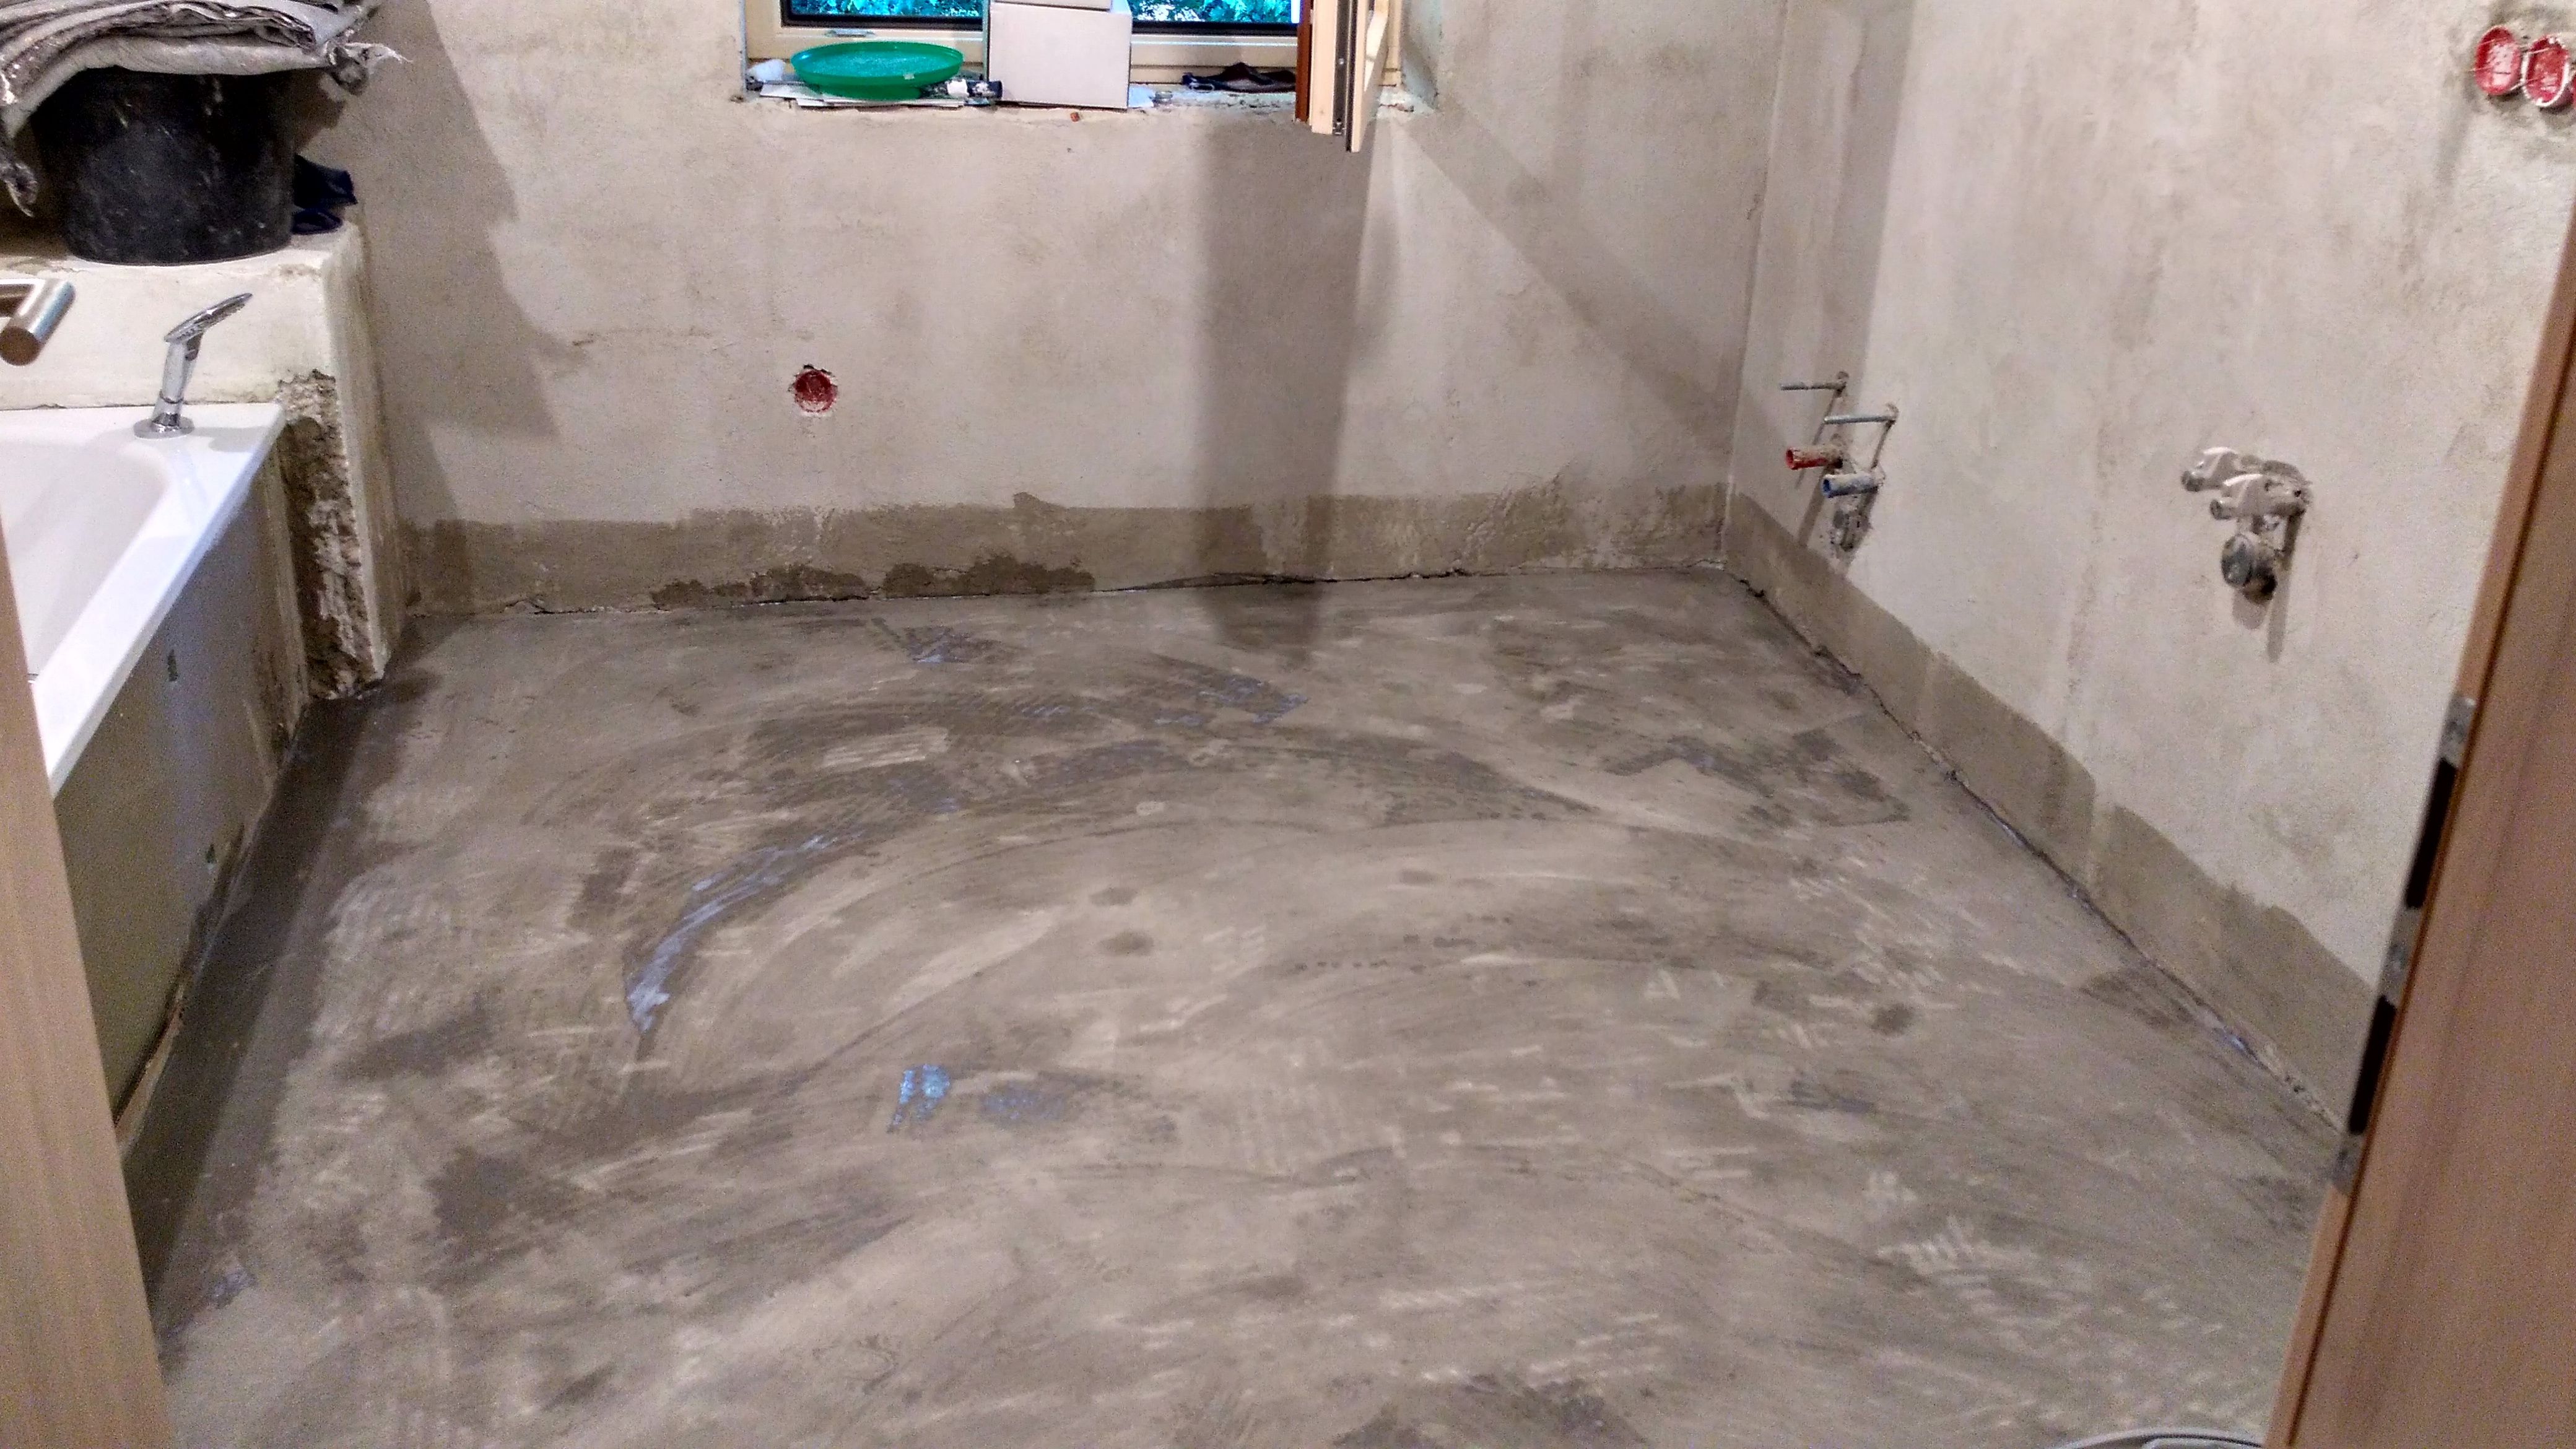
\includegraphics[scale=0.1]{Resources/Praktikum/IMG_20180801_090215_HDR.jpg}
		\caption{Rohbau}	
	\end{center}
\end{figure}

\begin{figure}[h]
	\begin{center}
		\noindent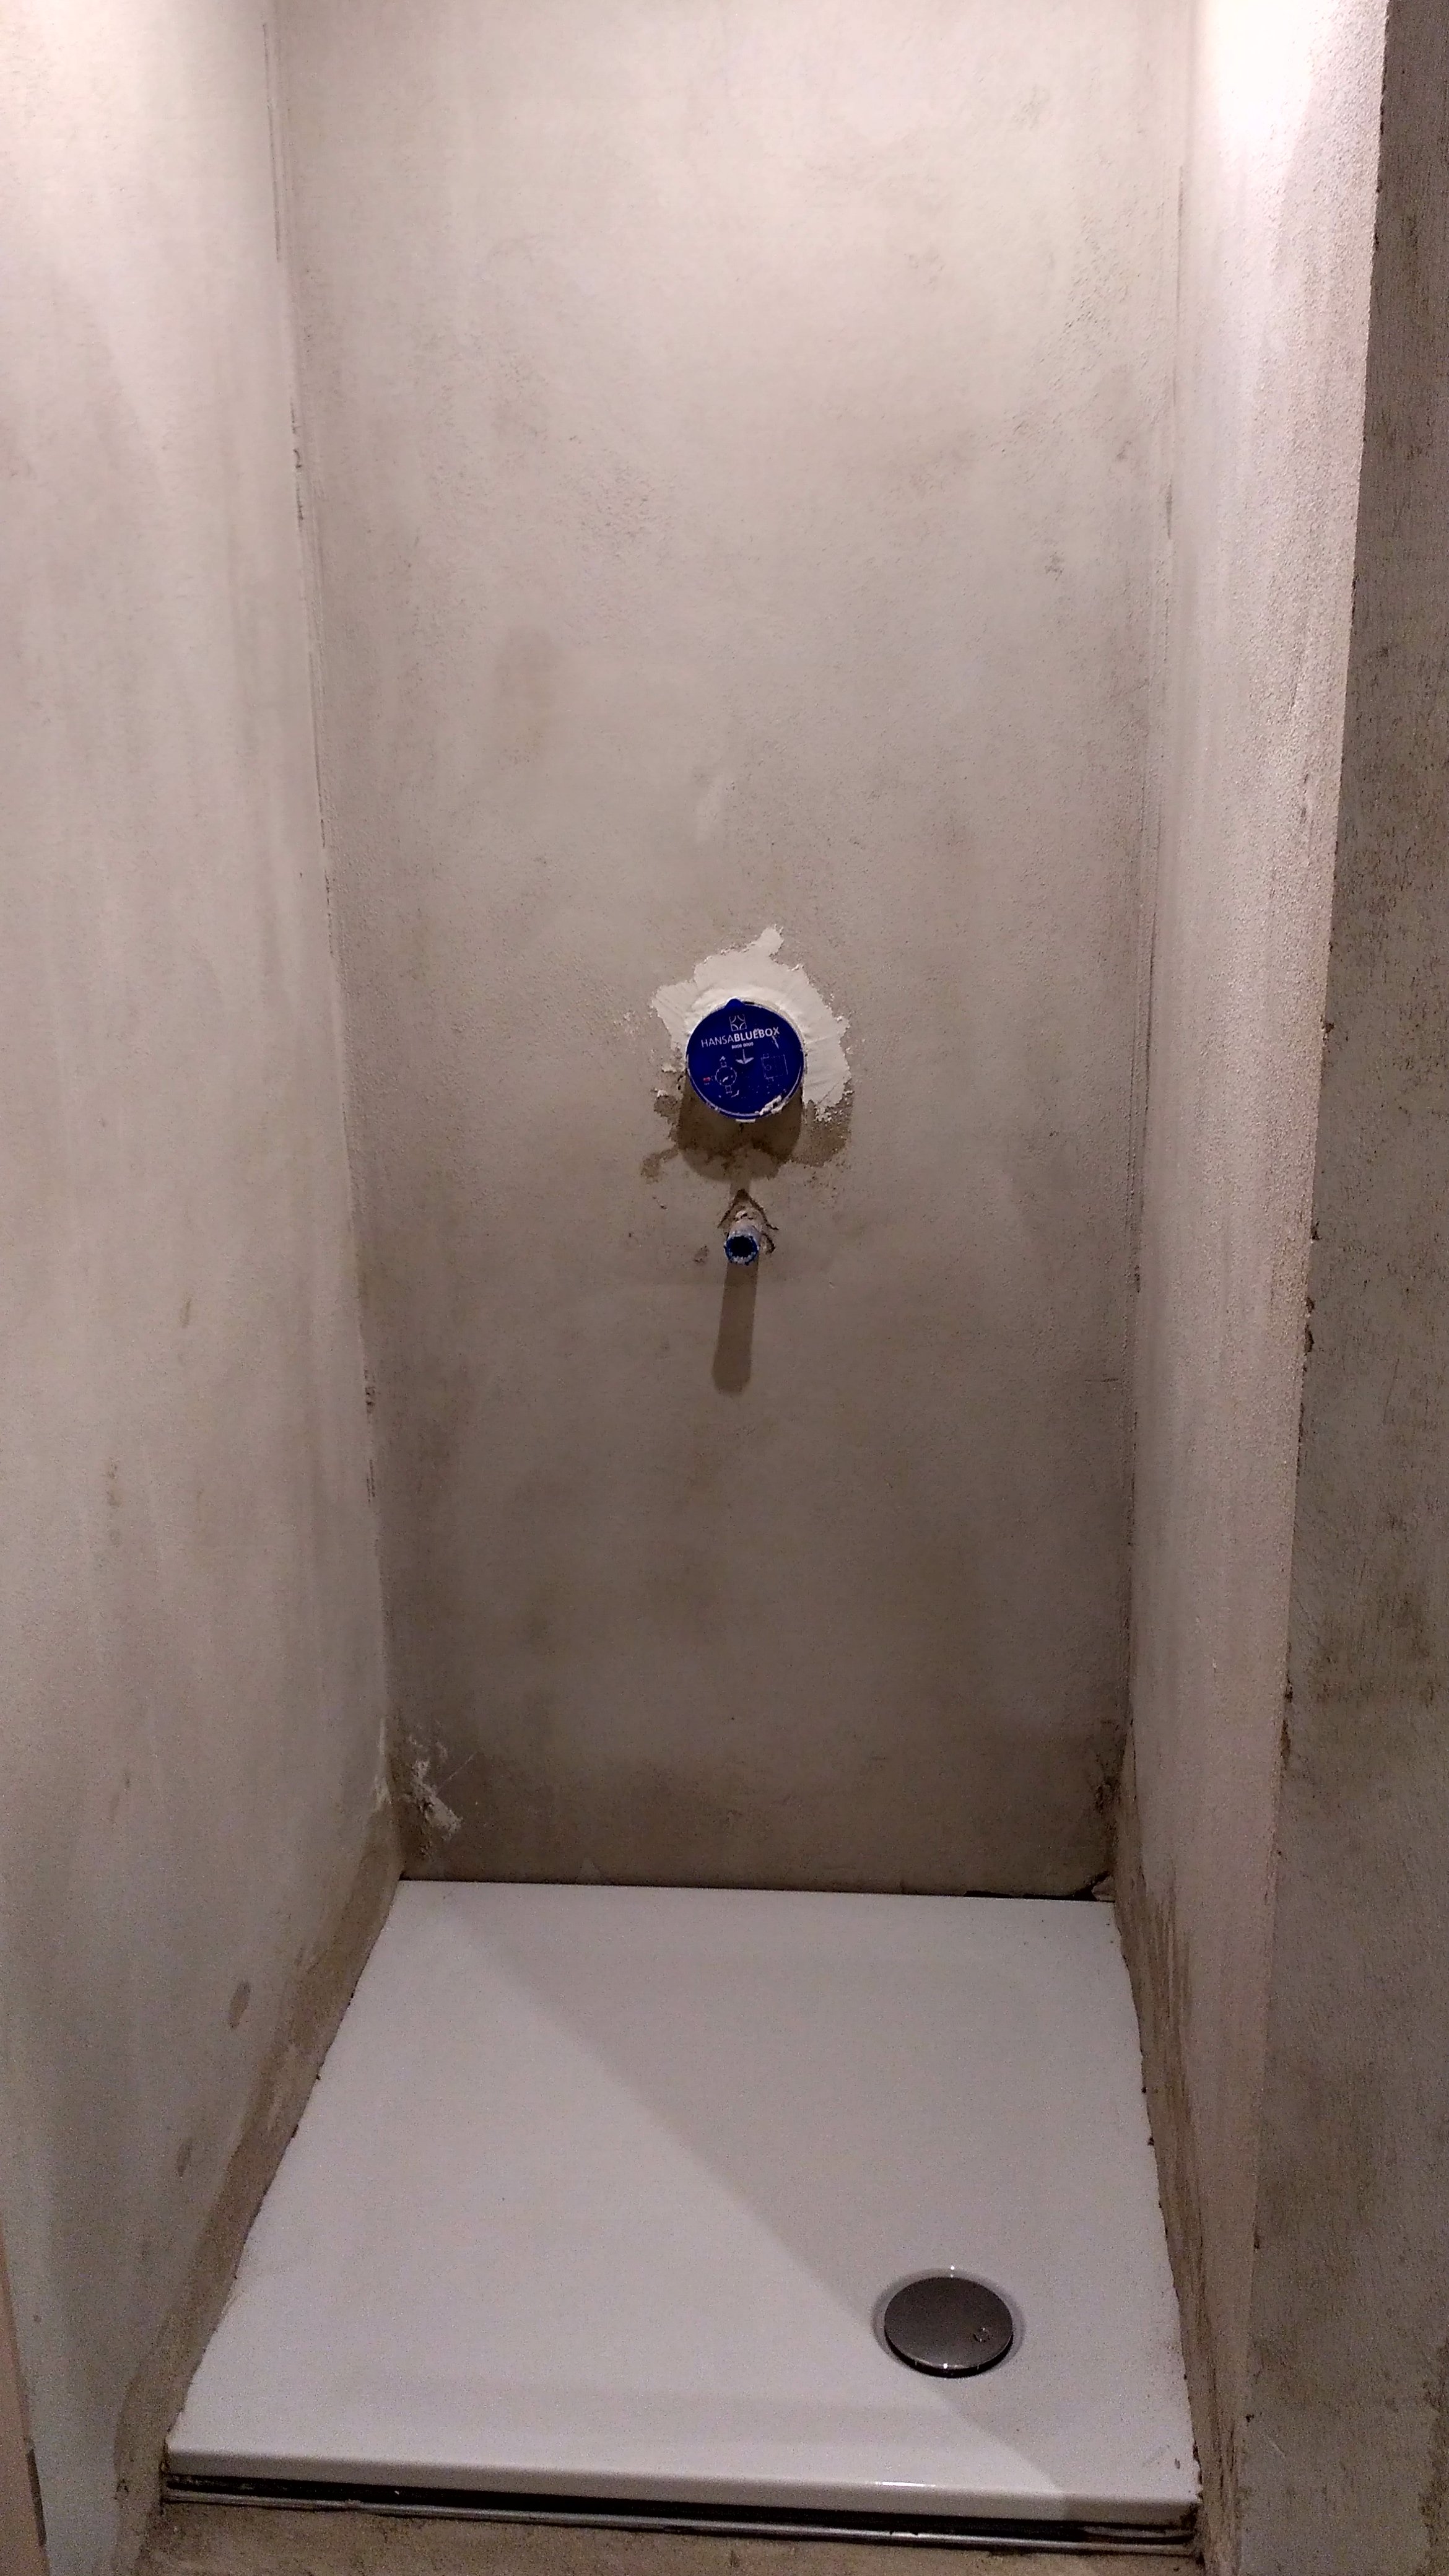
\includegraphics[scale=0.1]{Resources/Praktikum/IMG_20180731_085142_HDR.jpg}
		\caption{Rohbau: Dusche}	
	\end{center}
\end{figure}

\begin{figure}[h]
	\begin{center}
		\noindent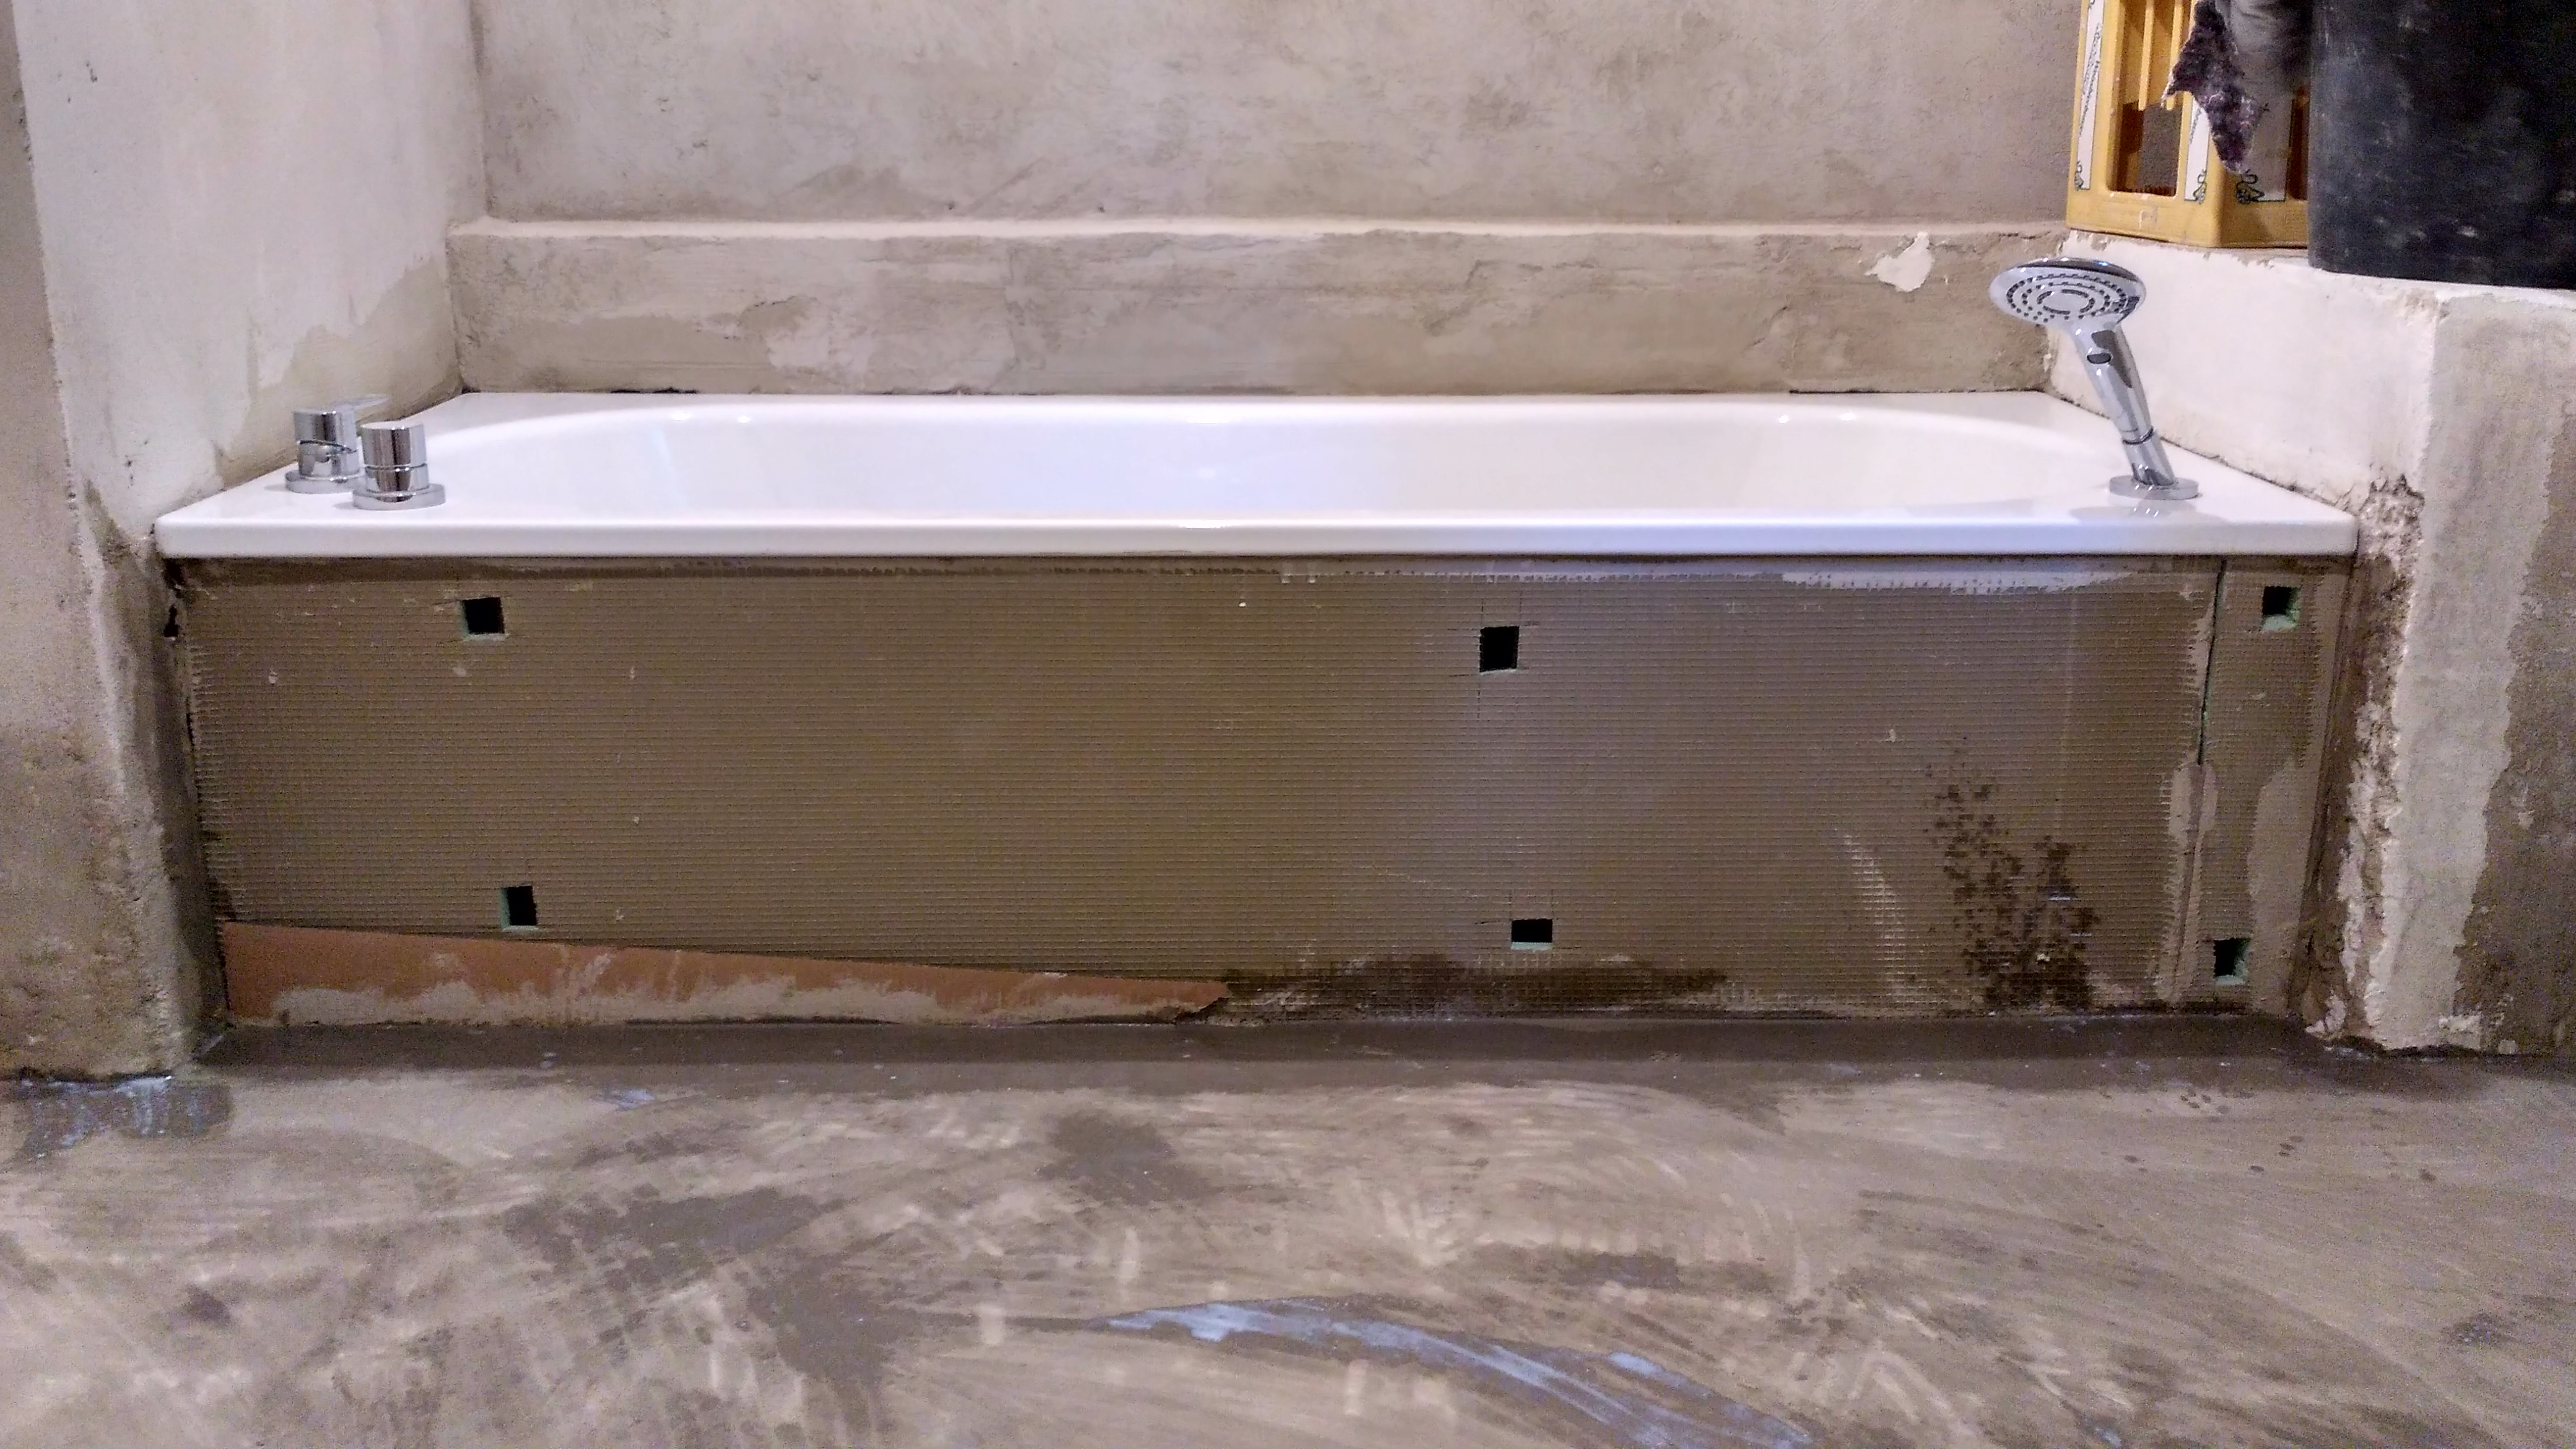
\includegraphics[scale=0.1]{Resources/Praktikum/IMG_20180801_090144_HDR.jpg}
		\caption{Rohbau: Badewanne mit eingesetzter Bauplatte}	
	\end{center}
\end{figure}

Zu Anfang führte uns der Kunde auf der Baustelle in den Rohbau des Bads, welches er verfliest und installiert haben wollte. Der Raum wurde bis jetzt nur von den Maurern verputzt. Nischen für eine Badewanne und eine Dusche waren jedoch schon vorgesehen. Die Wannen dafür waren bereits in den Nischen positioniert. Der Kunde wollte 20x30cm Fliesen im Raum verlegen, welche er uns im Katalog zeigte, und fragte den Fliesenleger nach seiner Meinung. Dieser nahm darauf seinen Meterstab zur Hand und fing an die einzelnen Seitenwände des Raumes zu bestimmen. Dies nahm ca. 5 Minuten in Anspruch. Der Fliesenleger schlug dem Kunden anschließend vor die Fliesen diagonal im Raum zu verlegen, da das ein schönes Muster ergäbe. Der Kunde reagierte auf diesen Vorschlag skeptisch und meinte er könne sich das nicht vorstellen. Er war der Meinung es sähe besser aus die Fliesen parallel zu der Wand, welche man direkt vor sich sieht wenn man den Raum betritt, zu verlegen. Der Fliesenleger skizzierte den Raum nun auf seinem Block und zeichnete die zwei Muster, parallel oder diagonal, grob ein und zeigte es dem Kunden. Die Zeichnungen verdeutlichten die beiden Ideen etwas, waren aber keine genaue Darstellung des Endergebnisses, nur eine Idee. Daraufhin begann eine rege Diskussion zwischen Fliesenleger und Kunde. Der Kunde war von seiner Idee überzeugt, stellte sich an verschiedene Punkte im Raum und schilderte seine Gedanken, woraufhin der Fliesenleger versuchte Vor- und Nachteile der Idee herauszuarbeiten. Am Ende einigten sie sich auf die Variante, die vom Kunden gewünscht wurde.

Laut dem Fliesenleger muss man die Wandfliesen an den Boden anpassen. Daher sollen auch diese horizontal zum Boden verlegt werden. Für die Wand sollen aber kleinere Fliesen verwendet werden.

\begin{figure}[h]
	\begin{center}
		\noindent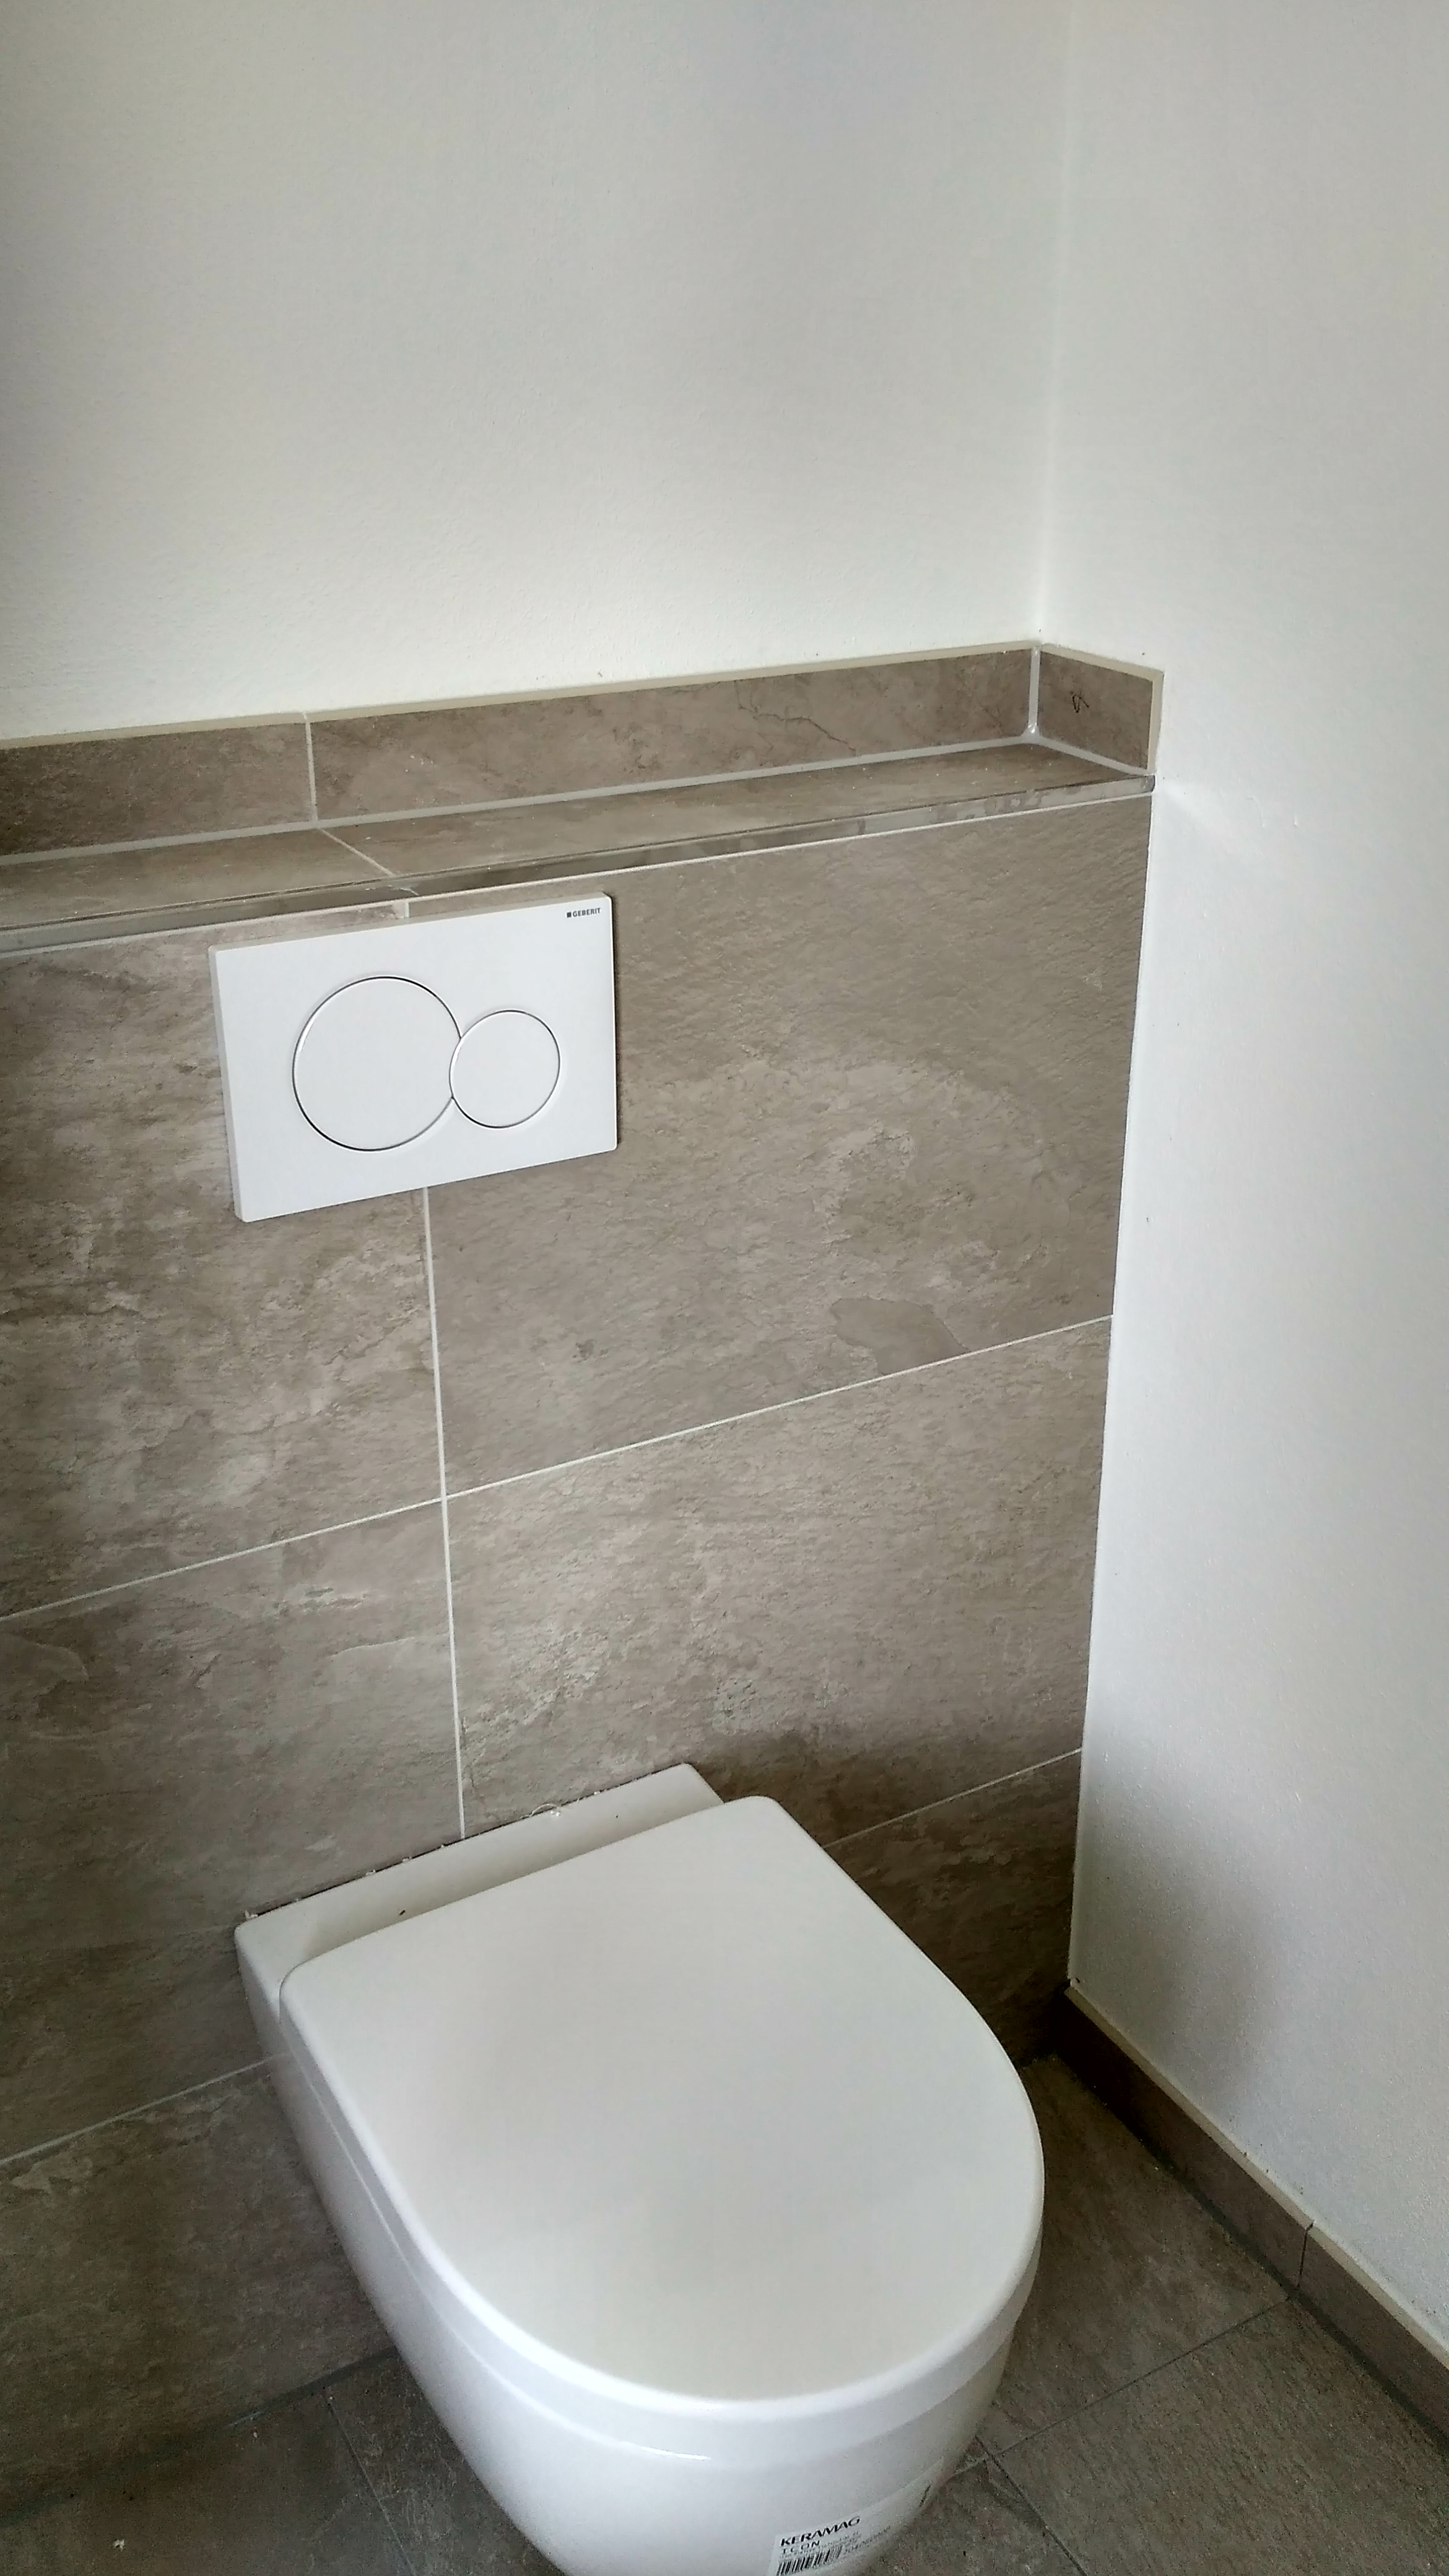
\includegraphics[scale=0.1]{Resources/Praktikum/IMG_20180801_131918_HDR.jpg}
		\label{toilette}
		\caption{Toilettenkasten mit Sockelleiste}	
	\end{center}
\end{figure}

\begin{figure}[h]
	\begin{center}
		\noindent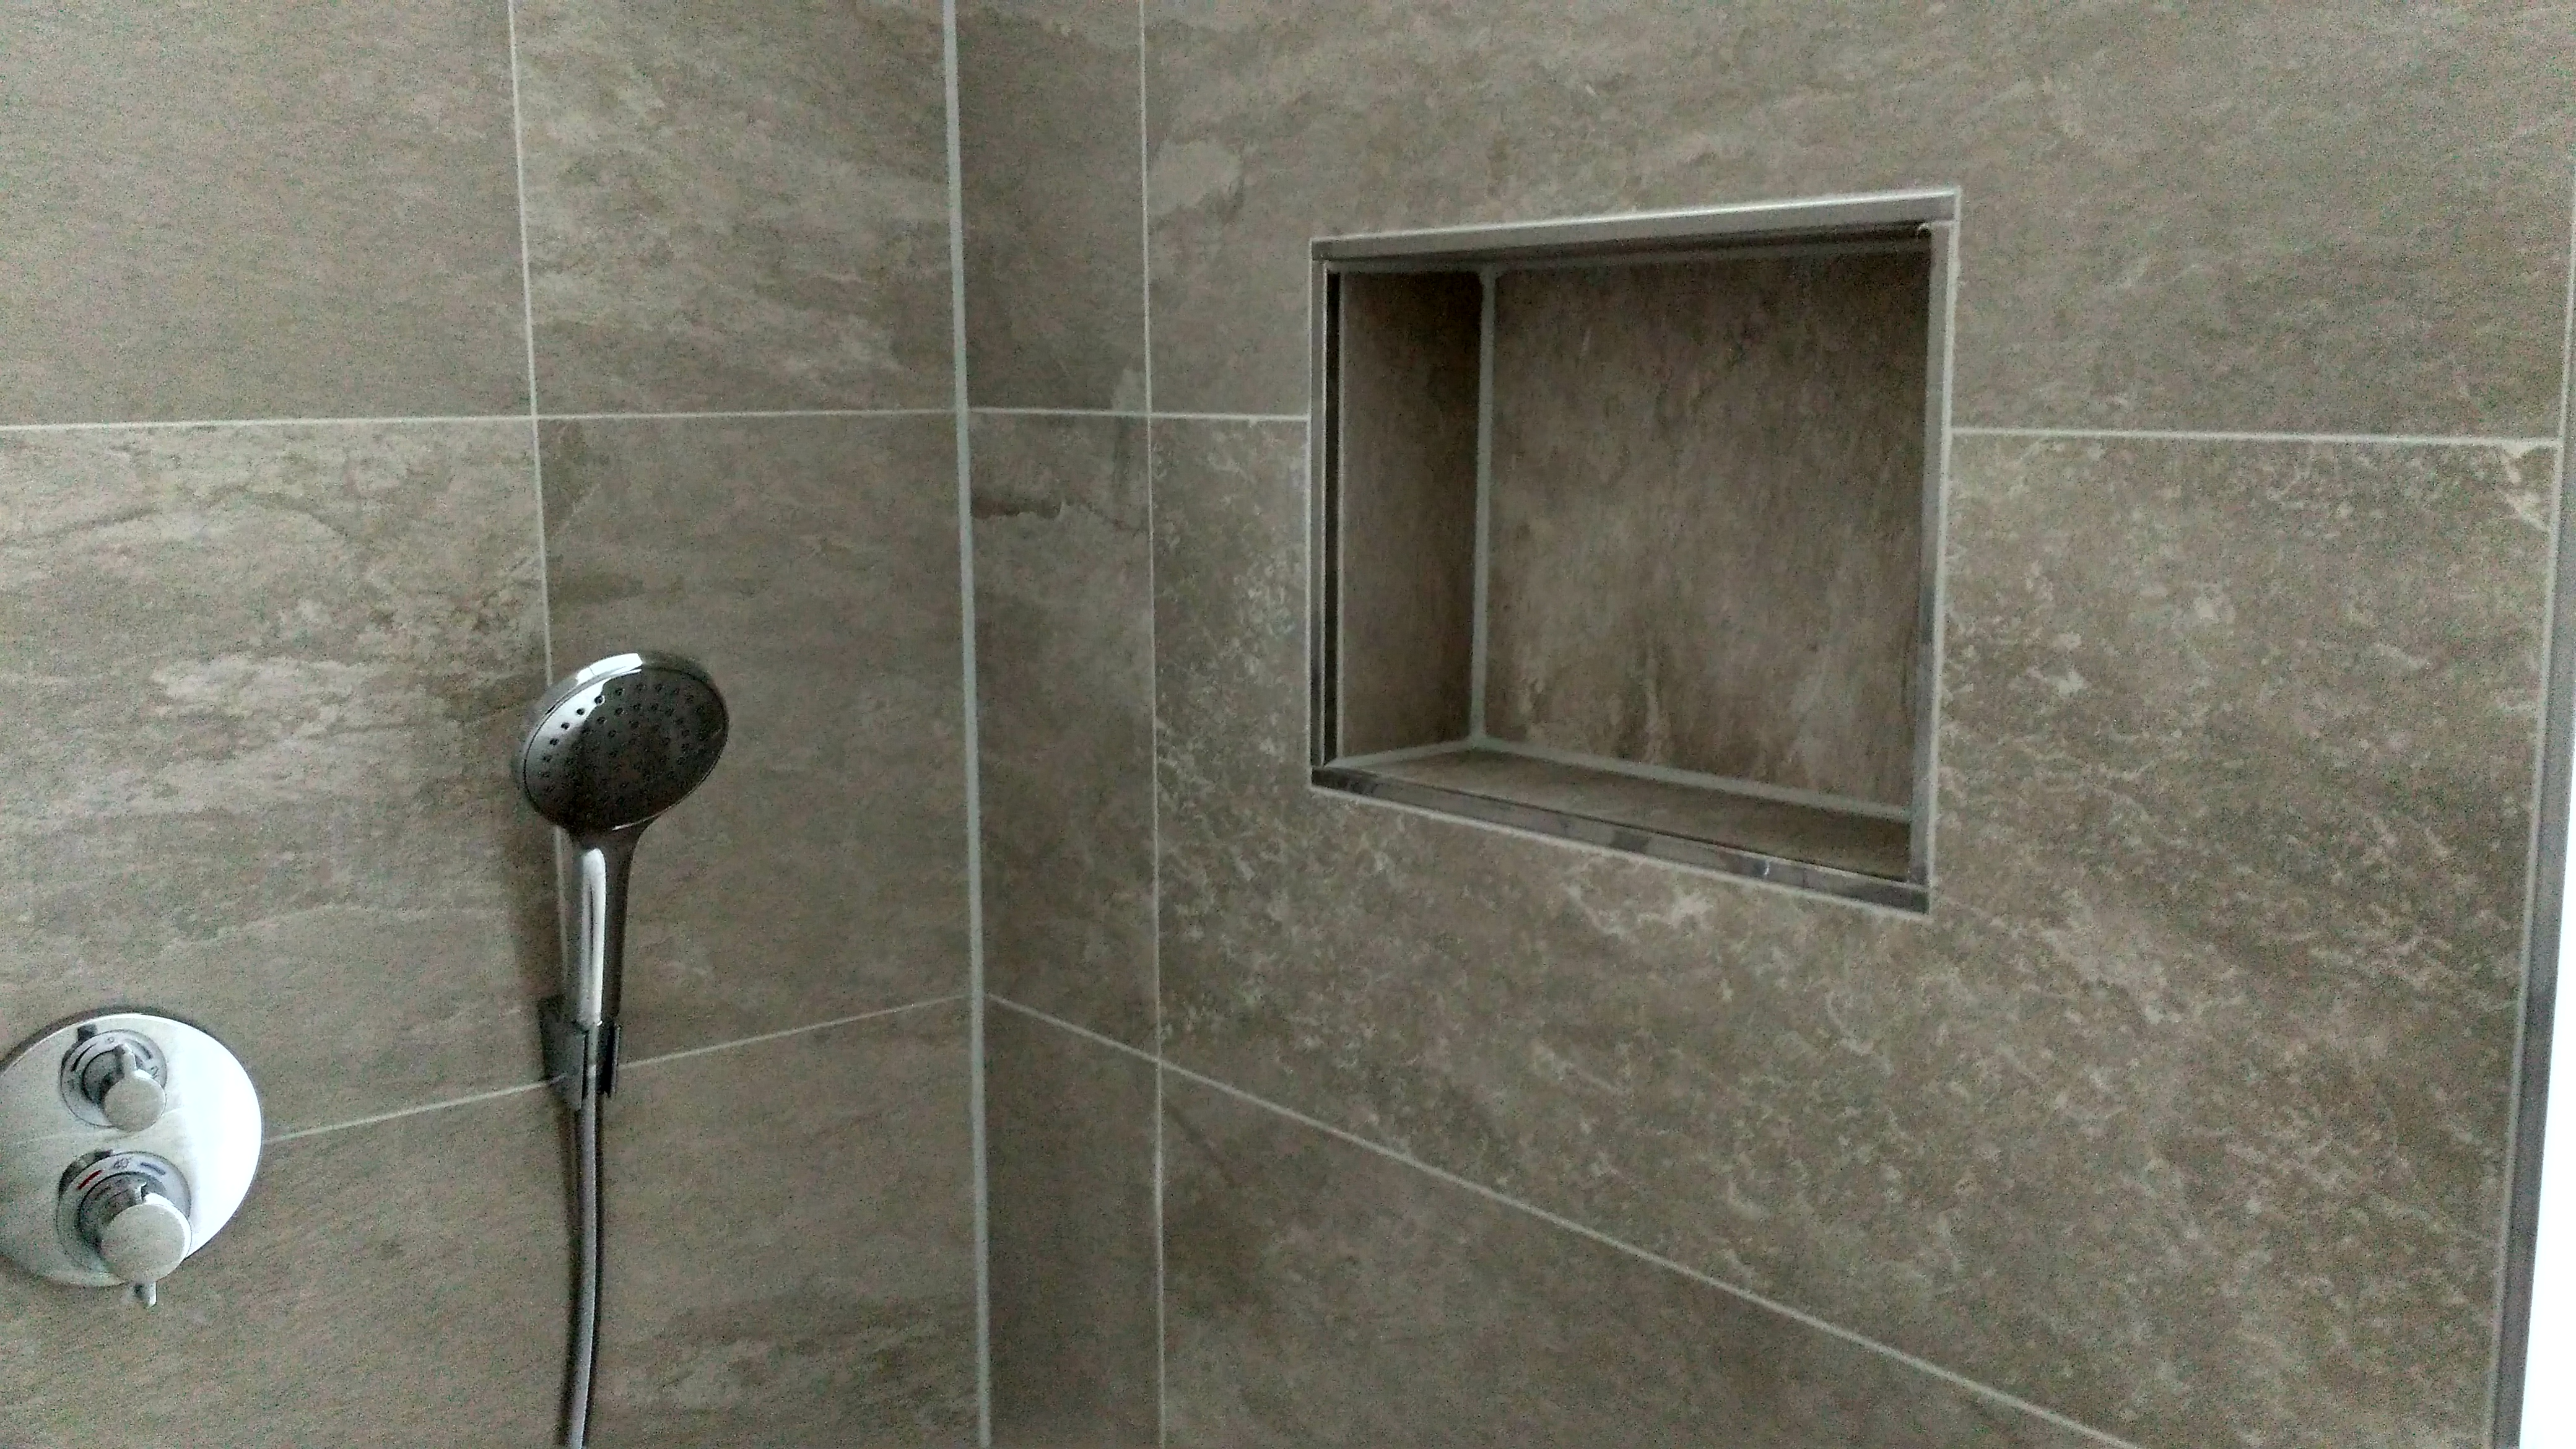
\includegraphics[scale=0.1]{Resources/Praktikum/IMG_20180801_132004_HDR.jpg}
		\label{duschenische}
		\caption{Dusche mit verfliester Abstellnische}	
	\end{center}
\end{figure}

\begin{figure}[h]
	\begin{center}
		\noindent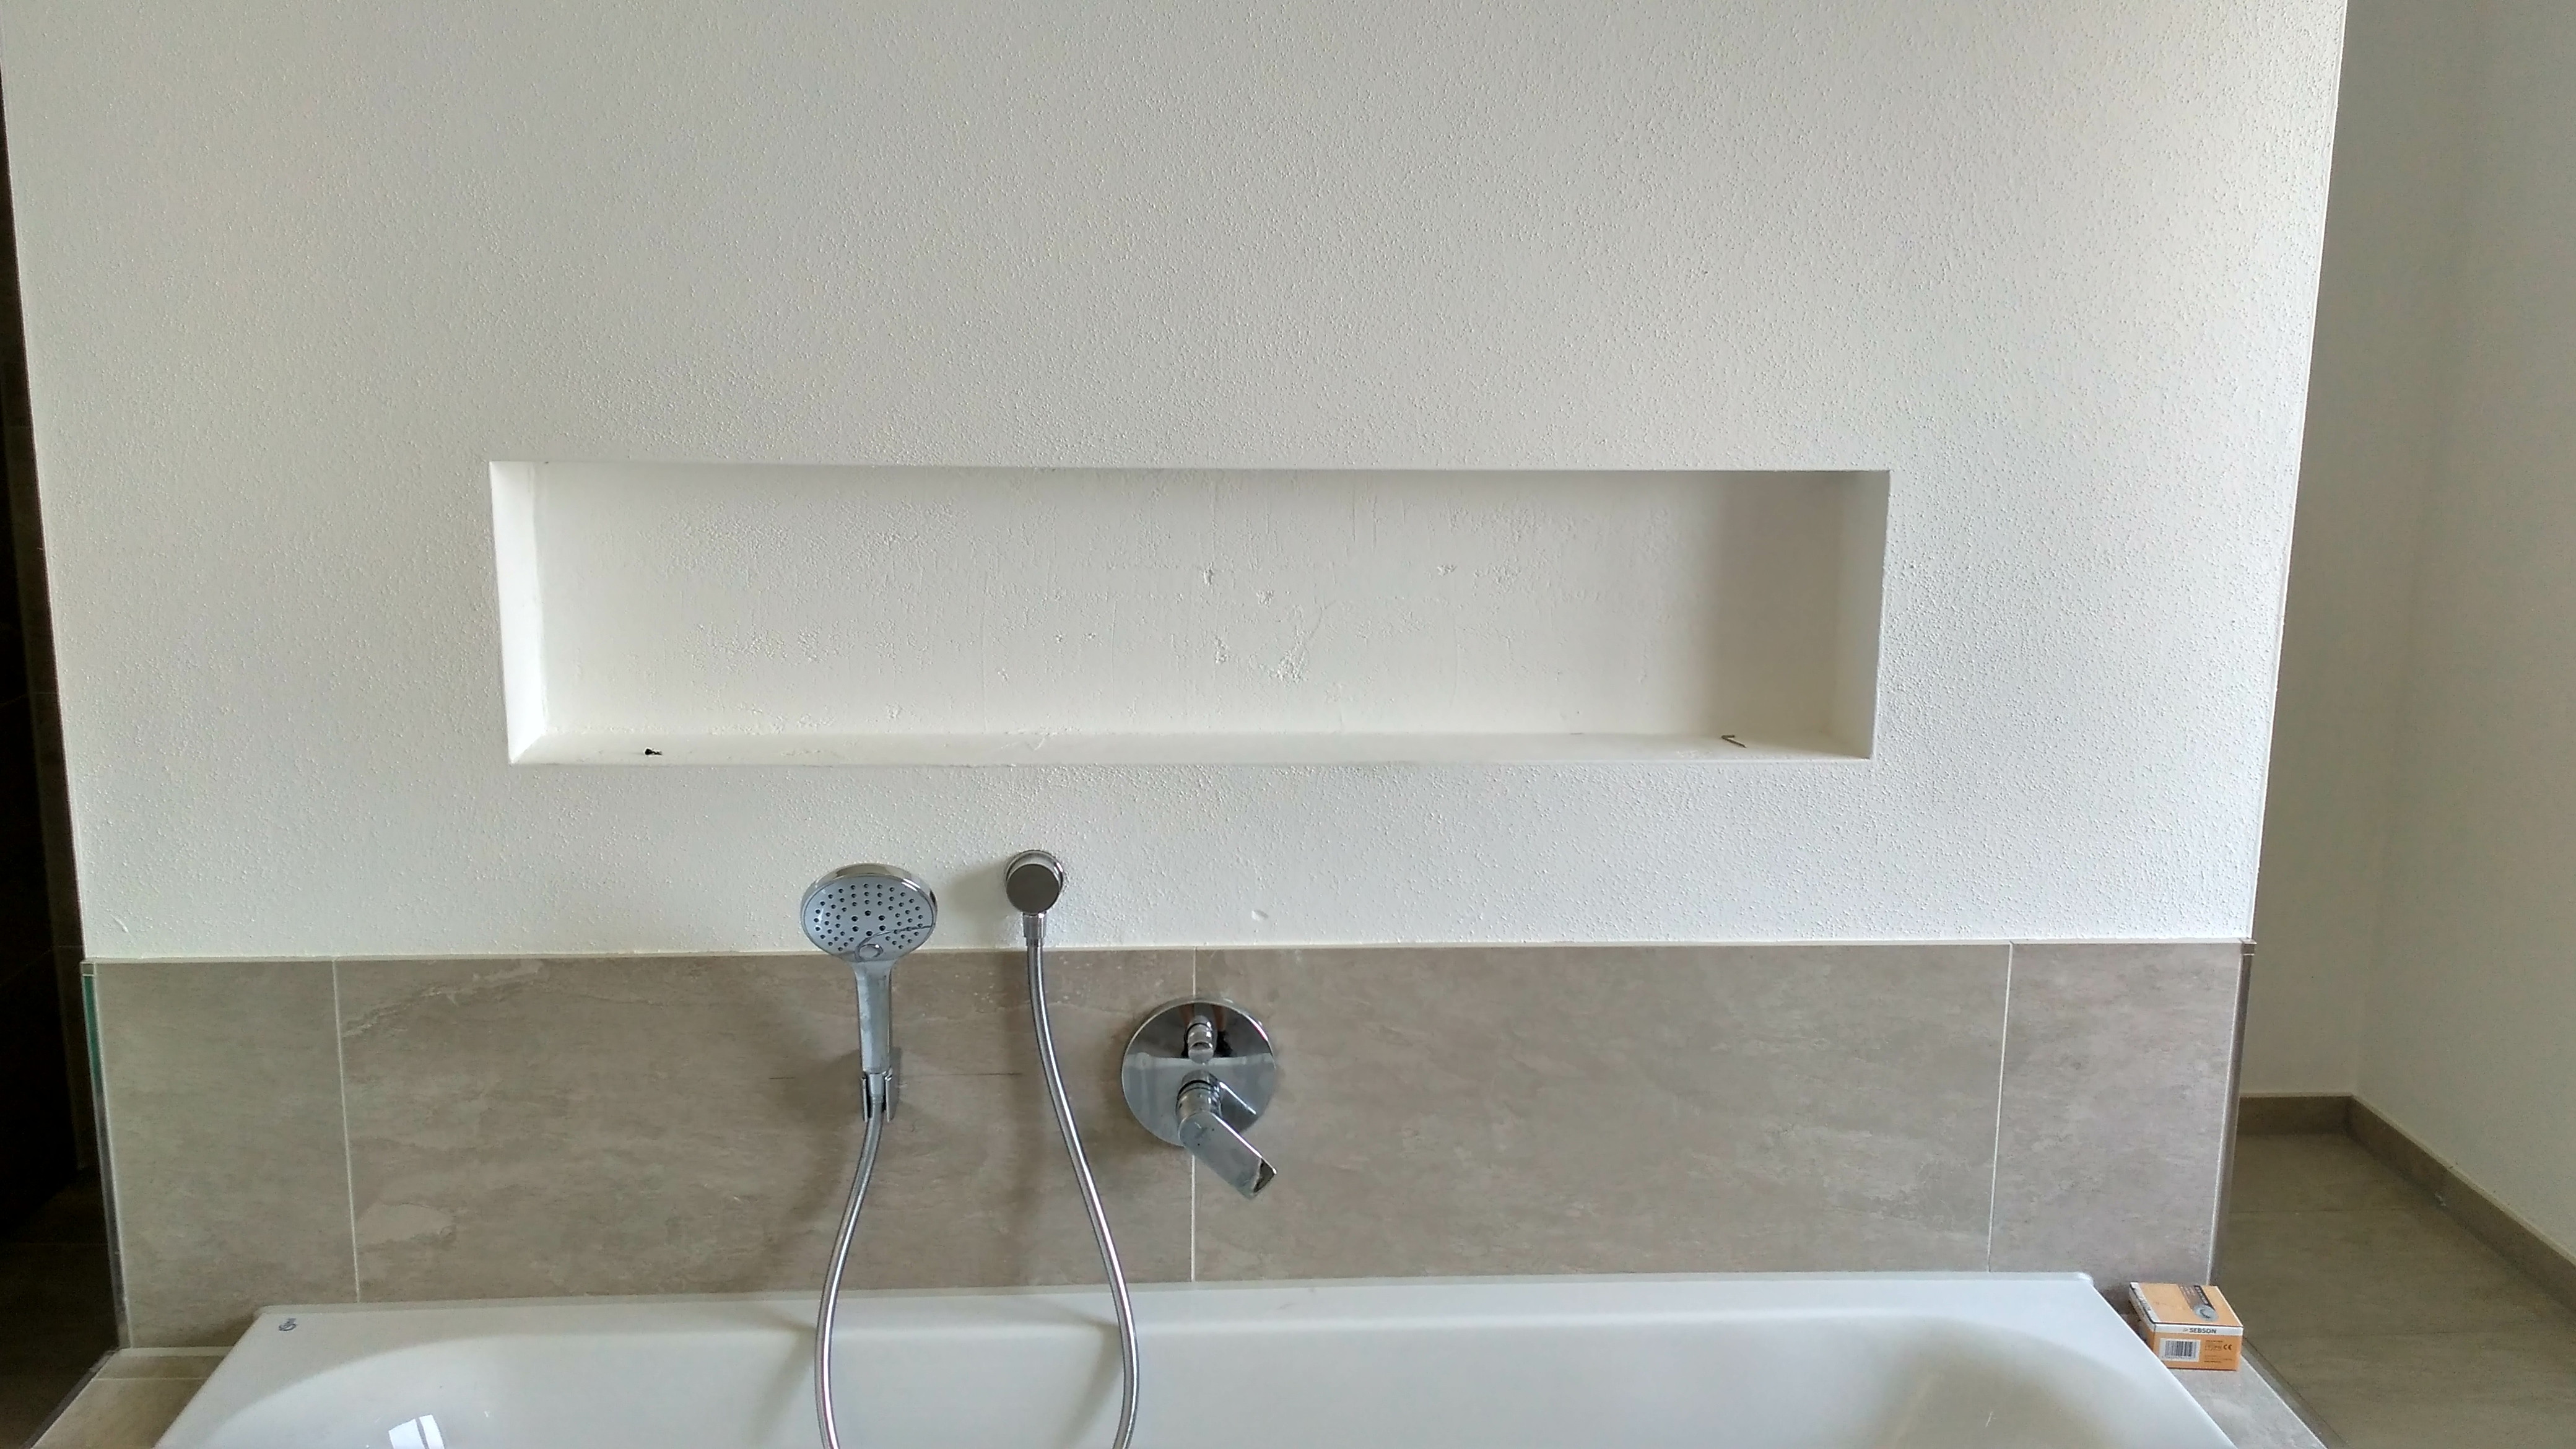
\includegraphics[scale=0.1]{Resources/Praktikum/IMG_20180801_131945_HDR.jpg}
		\label{wannenische}
		\caption{Badewanne mit nicht verfliester Abstellnische}	
	\end{center}
\end{figure}

\begin{figure}[h]
	\begin{center}
		\noindent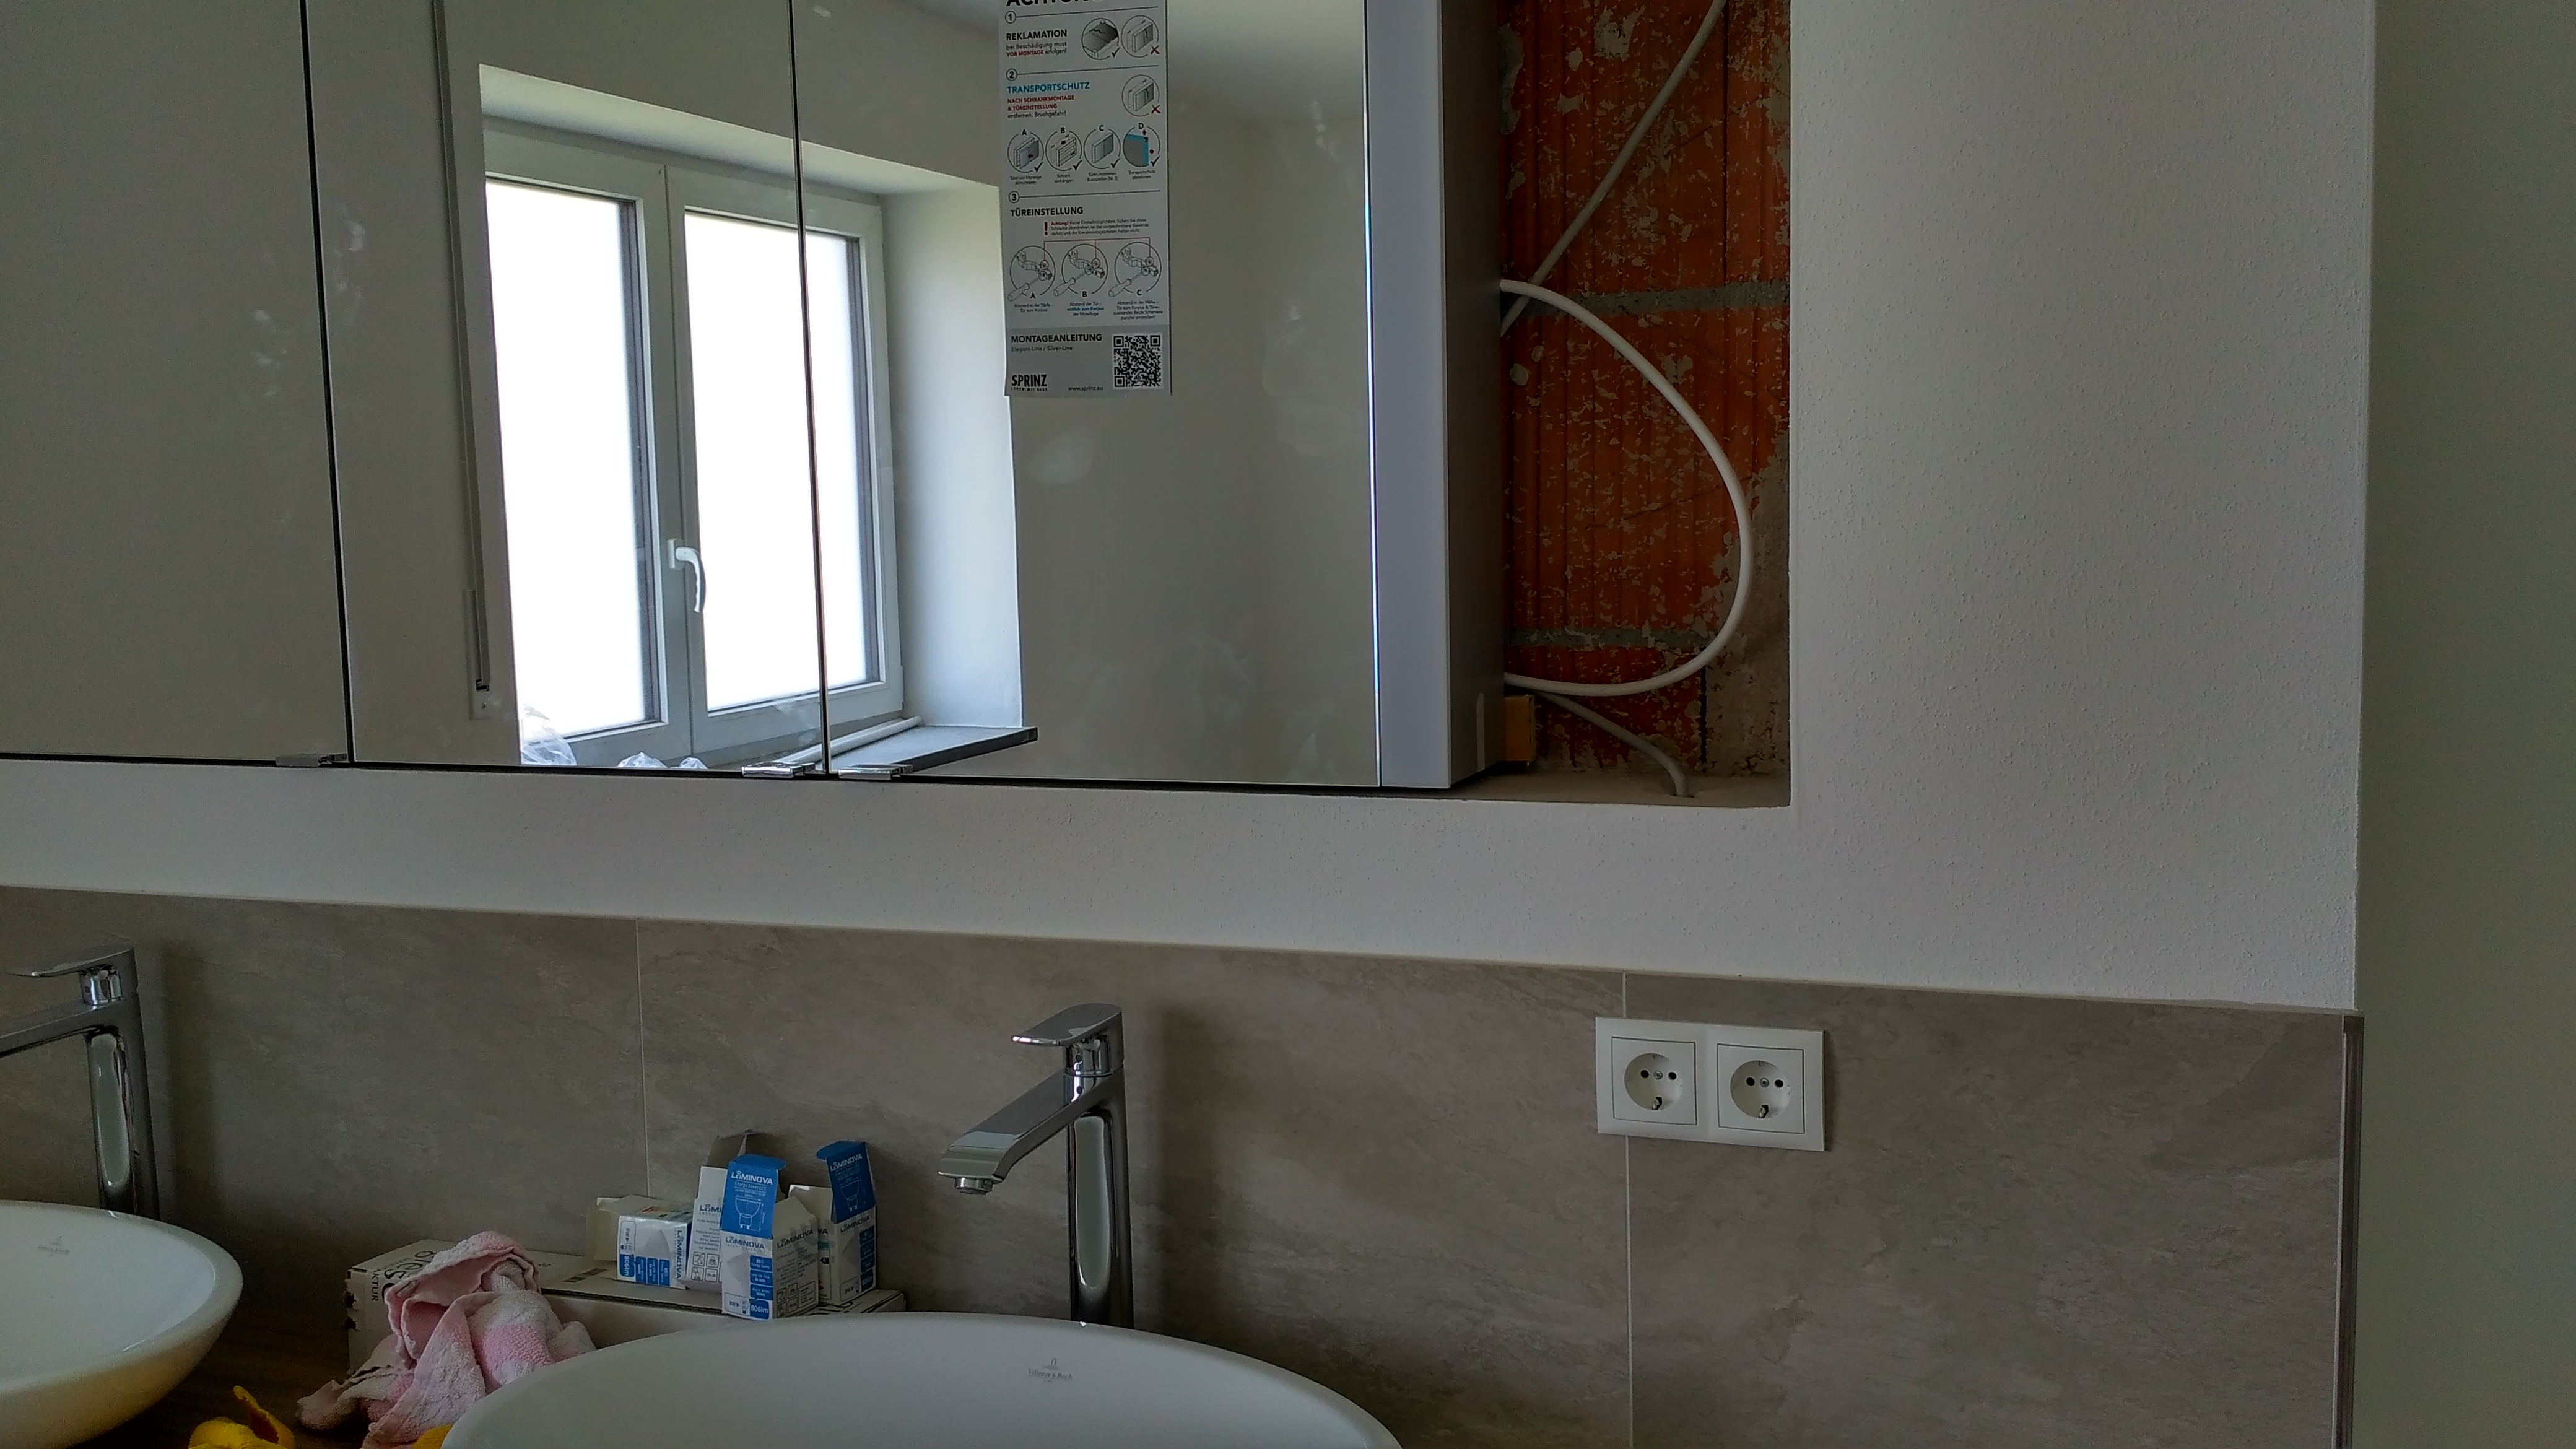
\includegraphics[scale=0.1]{Resources/Praktikum/IMG_20180801_131936_HDR.jpg}
		\label{waschbecken}
		\caption{Waschbecken mit nicht komplett verfliester Wand}	
	\end{center}
\end{figure}

Anschließend besprachen sie noch Details. Der Kunde wollte auf dem eingemauerten Spülkasten der Toilette keine Sockelleisten an der Wand anbringen. Der Fliesenleger überzeugte ihn jedoch vom Gegenteil, da sonst beim Putzen der Ablage leicht Feuchtigkeit an die verputzte Wand gelangen konnte (siehe Abbildung \ref{toilette}). Aus dem gleichen Grund riet er ihm die Nische in der Dusche, welche zum Abstellen von Duschgel gedacht ist, komplett zu verfliesen (siehe Abbildung \ref{duschenische}). Bei der Abstellnische neben der Badewanne beharrte der Kunde jedoch darauf, das diese nicht verfliest werden sollte, da es so besser aussähe (siehe Abbildung \ref{wannenische}). Er ließ sich auch von dem Argument, dass man dadurch immer Feuchtigkeit direkt auf der verputzten Mauer hat, was nicht gut ist, nicht überzeugen. Auch am Waschbecken wollte er die Wand nicht bis weit über das Waschbecken verfliest haben (siehe Abbildung \ref{waschbecken}). Dadurch entsteht die Gefahr von Feuchtigkeit auf der Wand durch Spritzwasser.

Bei diesem Kundengespräch fiel mir auf, dass es sehr unkoordiniert ablief. Die beiden Parteien redeten oft aneinander vorbei oder wiederholten ihre Gedanken, in der Hoffnung, dass ihr Gegenüber es dadurch besser versteht. Am deutlichsten wurde das bei dem Vorschlag des Fliesenlegers, die Fliesen diagonal zu verlegen. Mir kam es so vor, als könnte der Kunde sich das Muster im leeren Raum nicht vorstellen und reagierte deshalb mit Abneigung auf den Vorschlag. Ich selbst konnte es mir auch schlecht ausmalen und hätte mich hier auf den Fachmann und sein geschultes Auge verlassen müssen. Später fragte ich den Fliesenleger dazu, woraufhin er mir erklärte, dass Kunden tatsächlich wenig Vorstellungskraft besitzen, um sich komplett auf neue Vorschläge einzulassen, sich diese Vorzustellen und sie in Betracht ziehen, bei der Planung ihres Bads oder anderer Räume. Das erschwert die Kommunikation zwischen Experten und Kunden. Dadurch haben Kunde und Fliesenleger nach dem Gespräch oft unterschiedliche Vorstellungen im Kopf. Dann ist der Plan nicht genau festgelegt, was zu fehlerhafter Ausführung des Vertrags führen kann.

\subsection{Planung: Material}

Da festgelegt ist, wie die Fliesen verlegt werden sollen, geht es nun darum die Wandlängen und Winkel eindeutig zu bestimmen, festzulegen wo im Raum kritische Stellen, wie beispielsweise um ein Fenster, auftreten können, sowie wie viel Material an Fliesen, Kleber, Periplan und sonstigem gebraucht werden.

Dazu misst der Fliesenleger zuerst die Wände, um zu errechnen, wie viel Quadratmeter Bodenfläche der Raum hat. In diesem Raum, mit allen Einbuchtungen und Nischen dauerte das ca. 10 Minuten. Mit den daraus errechneten Quadratmetern kann er sich ein Bild machen, wie viel Material er zum präparieren des Bodens braucht. Da der Boden einen Riss aufweist, sollte auf diesen nicht direkt gefliest werden. Normalerweise würde man den Riss aufsägen und mit einer flexiblen Masse füllen. Unter dem verputzten Boden liegt jedoch eine Bodenheizung, welche das aufsägen zu gefährlich macht. Deshalb notiert sich der Fliesenleger auch Entkopplungsmatten für den gesamten Raum mitzubringen, welche man über den Riss legen kann, um das aufsägen zu umgehen. Zum Einmauern der Badewanne benötigt er noch eine Badewanne, wofür er sich die nötigen Maße notiert.

Der Fliesenleger erklärt mir, dass es gewisse Vorschriften für Bäder gibt, wie diese abgedichtet werden müssen. Ecken und Kanten am Boden, in der Dusche auch an der Wand, müssen mit Abdichtbändern beklebt werden. Die Wände der Dusche müssen zusätzlich noch mit Flüssigfolie ausgestrichen werden. Diese Maßnahmen dienen dazu, das Bad wasserundurchlässig zu machen und so Schimmel und ähnlichen Schäden vorzubeugen. Ein gefliester Boden gilt nicht als wasserdicht.

Aus den Quadratmetern des Raumes lässt sich leicht bestimmen, wie viele Fliesen benötigt werden. Der Fliesenleger überlegte sich, wo er mit dem Verlegen der Fliesen beginnen sollte. Dabei stellte er sich vor allem zwei Fragen:

\begin{itemize}
	\item Wie sieht das Ergebnis am besten aus?
	\item Wie minimiert man den Verschnitt?
\end{itemize}

Dazu sagte er mir, ganze Fliesen sehen am besten aus, weshalb er versucht diese im Blickfeld, beim Betreten des Raumes zu positionieren. Ganze Fliesen sehen immer ansprechender aus als geschnittene. Er maß aus, wie viele ganze Fliesen er nebeneinander legen konnte, und wie viel er von der Letzten in der Reihe abschneiden musste. Ungünstiger Verschnitt wären Fliesen von unter 1cm Breite, welchen er zu vermeiden versucht. Seine Abschätzung zeigte aber, dass die geschnittene Fliese mindestens 5cm Breit sein würde. Anschließend misst er die Winkel der Ecken genau. Haben diese nämlich keinen exakten 90 Grad Winkel, führt das später zu Ungleichmäßigkeiten am verlegten Boden, wenn er es nicht vorher entdeckt. Er merkte dabei an, dass er kleine Abweichungen von 90 Grad mit minimalen Änderungen der Fugenbreite ausgleichen kann. Sollte die Abweichung aber zu groß sein, funktioniert das nicht mehr. Dann läuft er Gefahr ungünstigen Verschnitt zu bekommen. Ungleichmäßige Materialien an den Wänden, wie beispielsweise Holzwände können dies noch verstärken.

Mit diesen Informationen legte der Fliesenleger fest, wie viele Fliesen und wie viel anderes Material wir für die Baustelle benötigten. 

\subsection{Vorbereitung des Raums}
 
Die Wände der Dusche waren unten nicht senkrecht verputzt worden. Über eine schiefe Wand kann man nicht fliesen, da es sonst unregelmäßig und bruchanfällig wird. Deshalb bestand meine erste Aufgabe darin den überflüssigen Putz mit Hammer und Meißel abzutragen. Durch Anlegen einer Wasserwage prüfte ich, ob die Wand wieder senkrecht war. Das war eine anstrengende Arbeit, die den halben Tag in Anspruch nahm. Dabei war die körperliche Komponente am zeitaufwendigsten. Danach schabte ich die Wände mit einem Metallschaber ab, um Mörtelreste zu entfernen und bestrich sie anschließend mit Grundierung. Diese bindet den Staub und sorgt dafür, dass darauf aufgetragene Baustoffe besser halten. Auch den gesamten Boden des Raums bestrich ich mit der Grundierung, nachdem ich ihn einmal gefegt hatte.

Währenddessen baute der Fliesenleger eine Bauplatte an der Seite der Badewanne ein. Dazu nahm er zuerst grob Maß und schnitt die Bauplatte zurecht. Das ging in weniger als einer Minute, da sie nicht genau passen muss, weil anschließend darüber gefliest wird und man Ungenauigkeiten nicht mehr sieht. Dann klebte er die Bauplatte mit Mörtel ein. Mit einer Wasserwage überprüfte er ob diese senkrecht zum Boden stand und korrigierte sie entsprechend. Danach klebte er, den Vorschriften für die Installation von Badewannen entsprechend, Abdichtbänder an deren Seiten ein. Da der Boden leichte Unebenheiten aufweisen kann, muss dieser noch geebnet werden. Dafür nutzt man Periplan, eine sehr flüssige Masse die der Fliesenleger mit einer gezahnten Kelle auf dem gesamten Boden verteilte. Durch ihren wässrigen Charakter breitete sie sich gleichmäßig auf dem Boden aus und ebnete ihn so. Wir ließen sie bis zum nächsten Tag anziehen. 

\begin{figure}[h]
	\begin{center}
		\noindent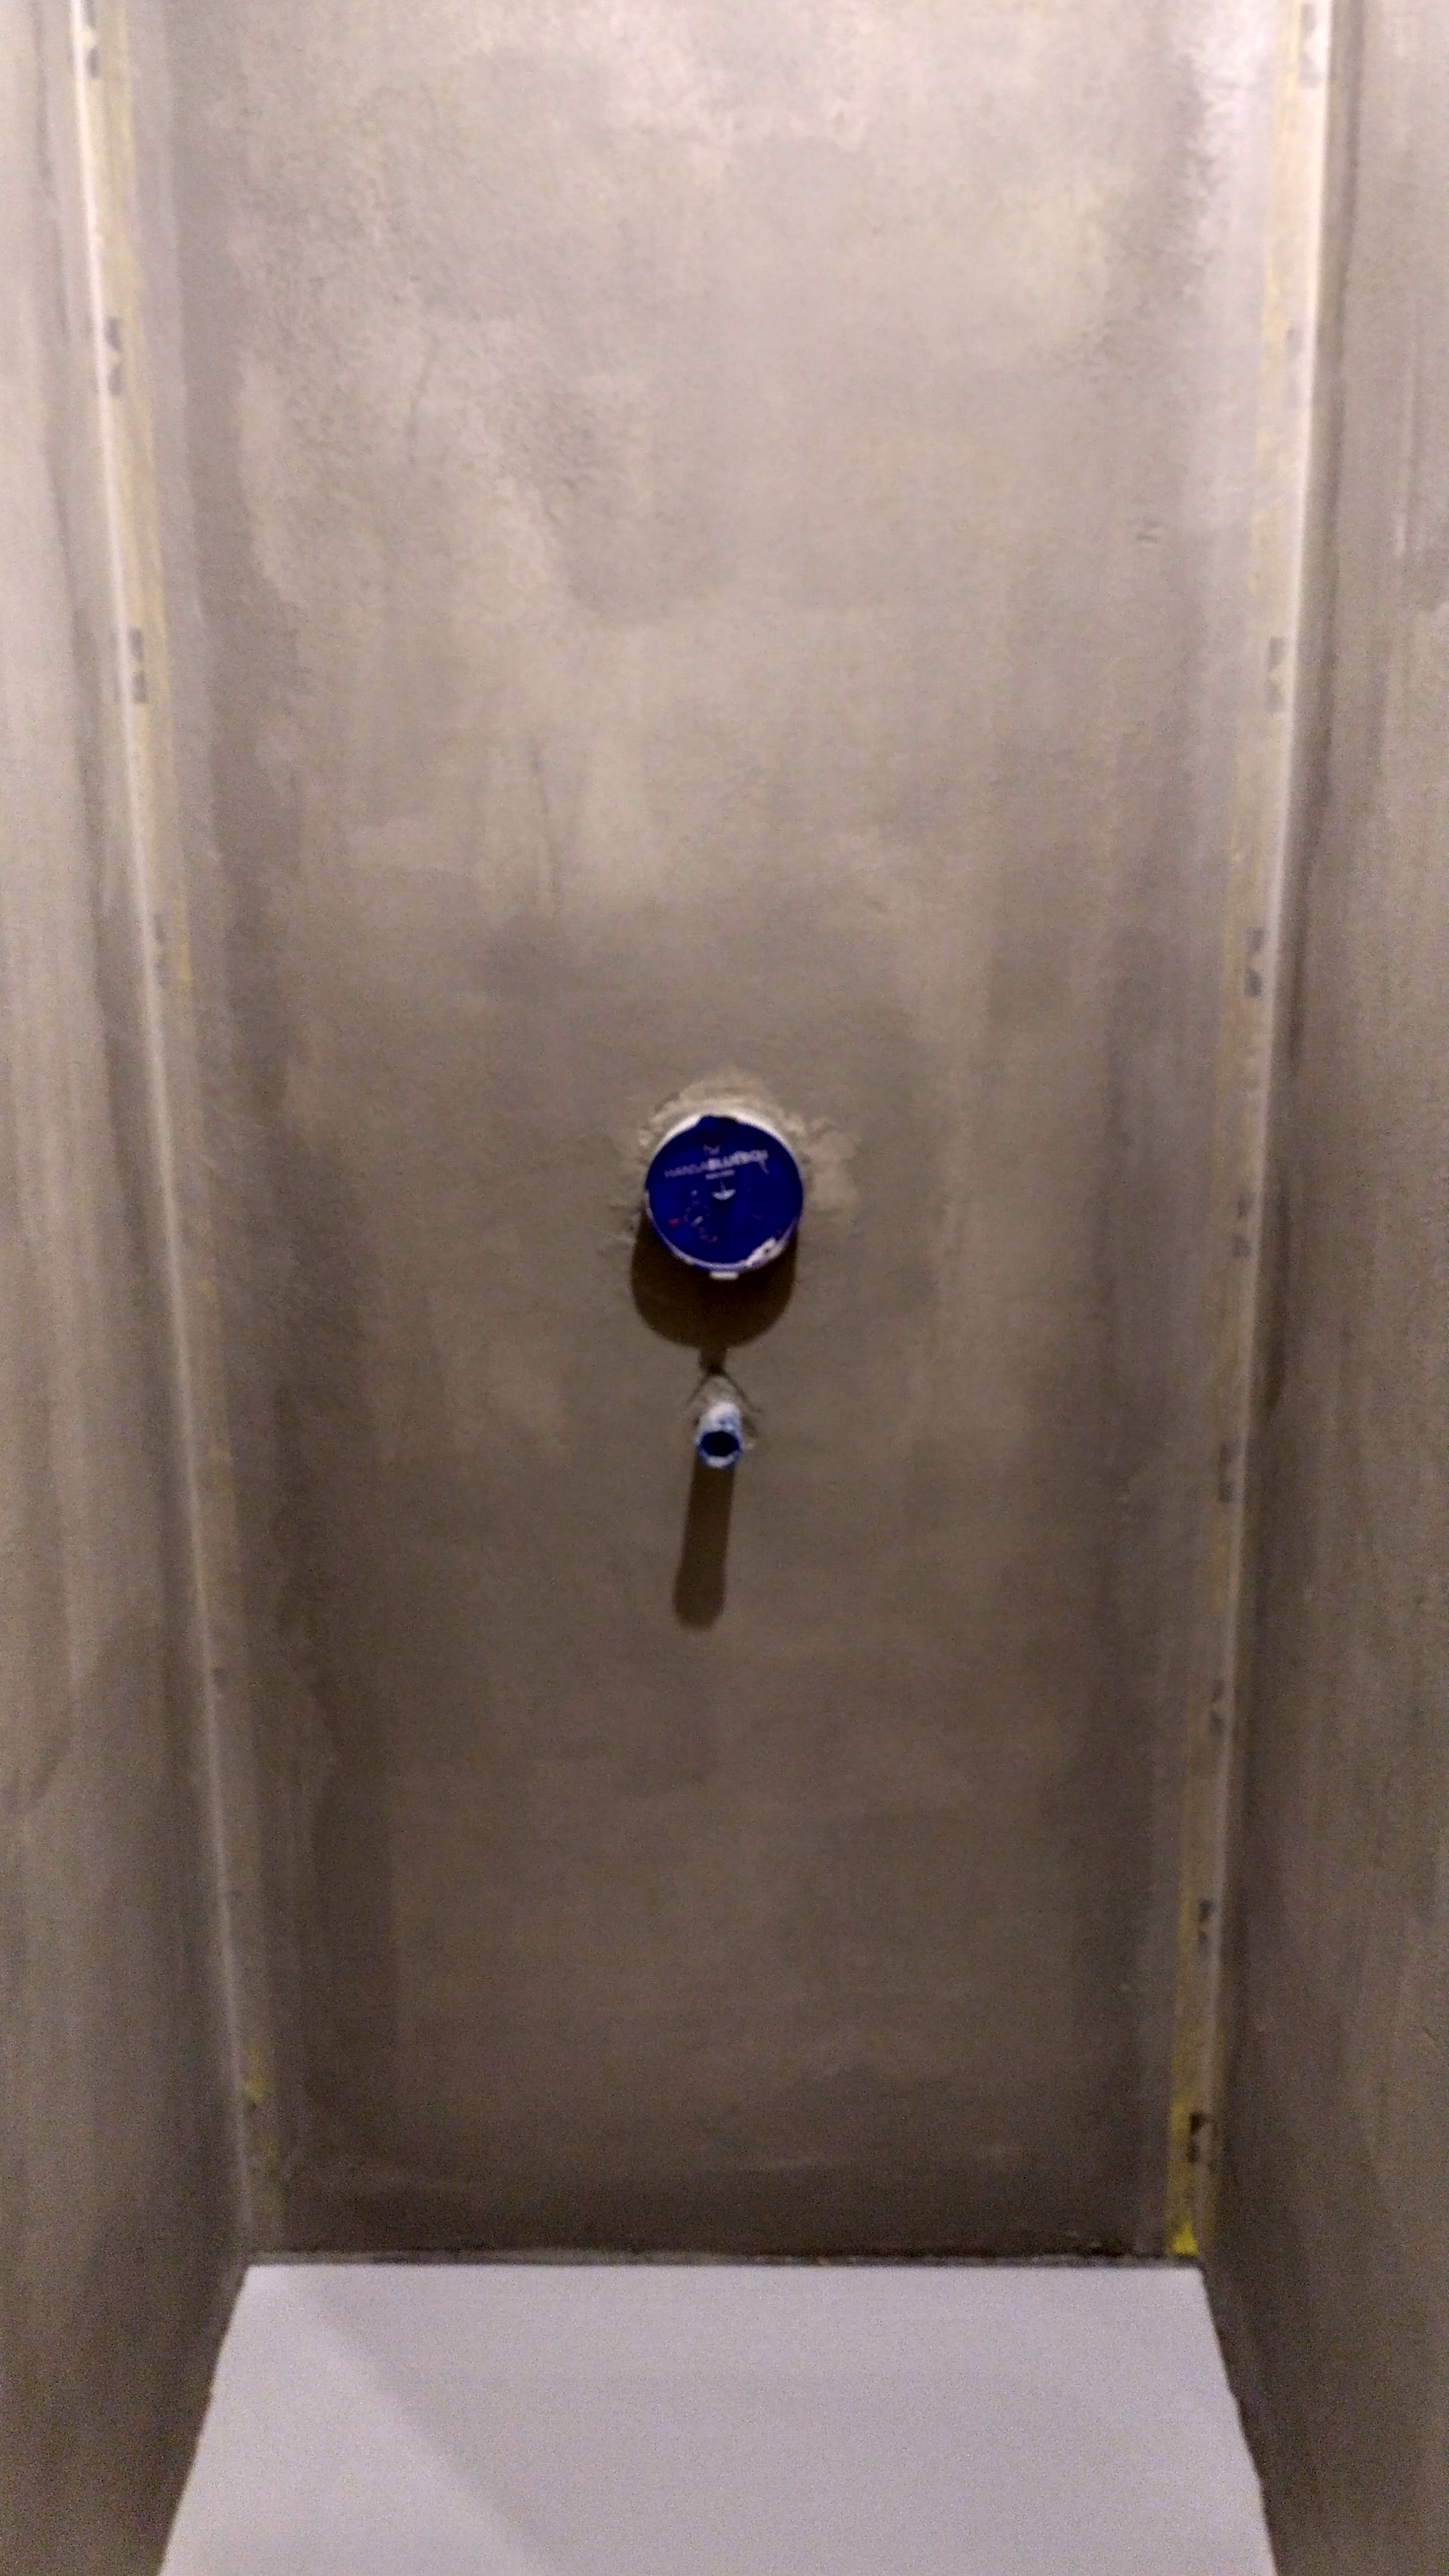
\includegraphics[scale=0.1]{Resources/Praktikum/IMG_20180801_114911_HDR.jpg}
		\label{duscheDicht}
		\caption{Abgedichtete Dusche}	
	\end{center}
\end{figure}

\begin{figure}[h]
	\begin{center}
		\noindent\includegraphics[scale=0.1]{Resources/Praktikum/IMG_20180801_114820_HDR.jpg}
		\label{bodenDicht}
		\caption{Boden mit Entkopplungsmatten und Abdichtbändern in den Ecken}	
	\end{center}
\end{figure}

\begin{figure}[h]
	\begin{center}
		\noindent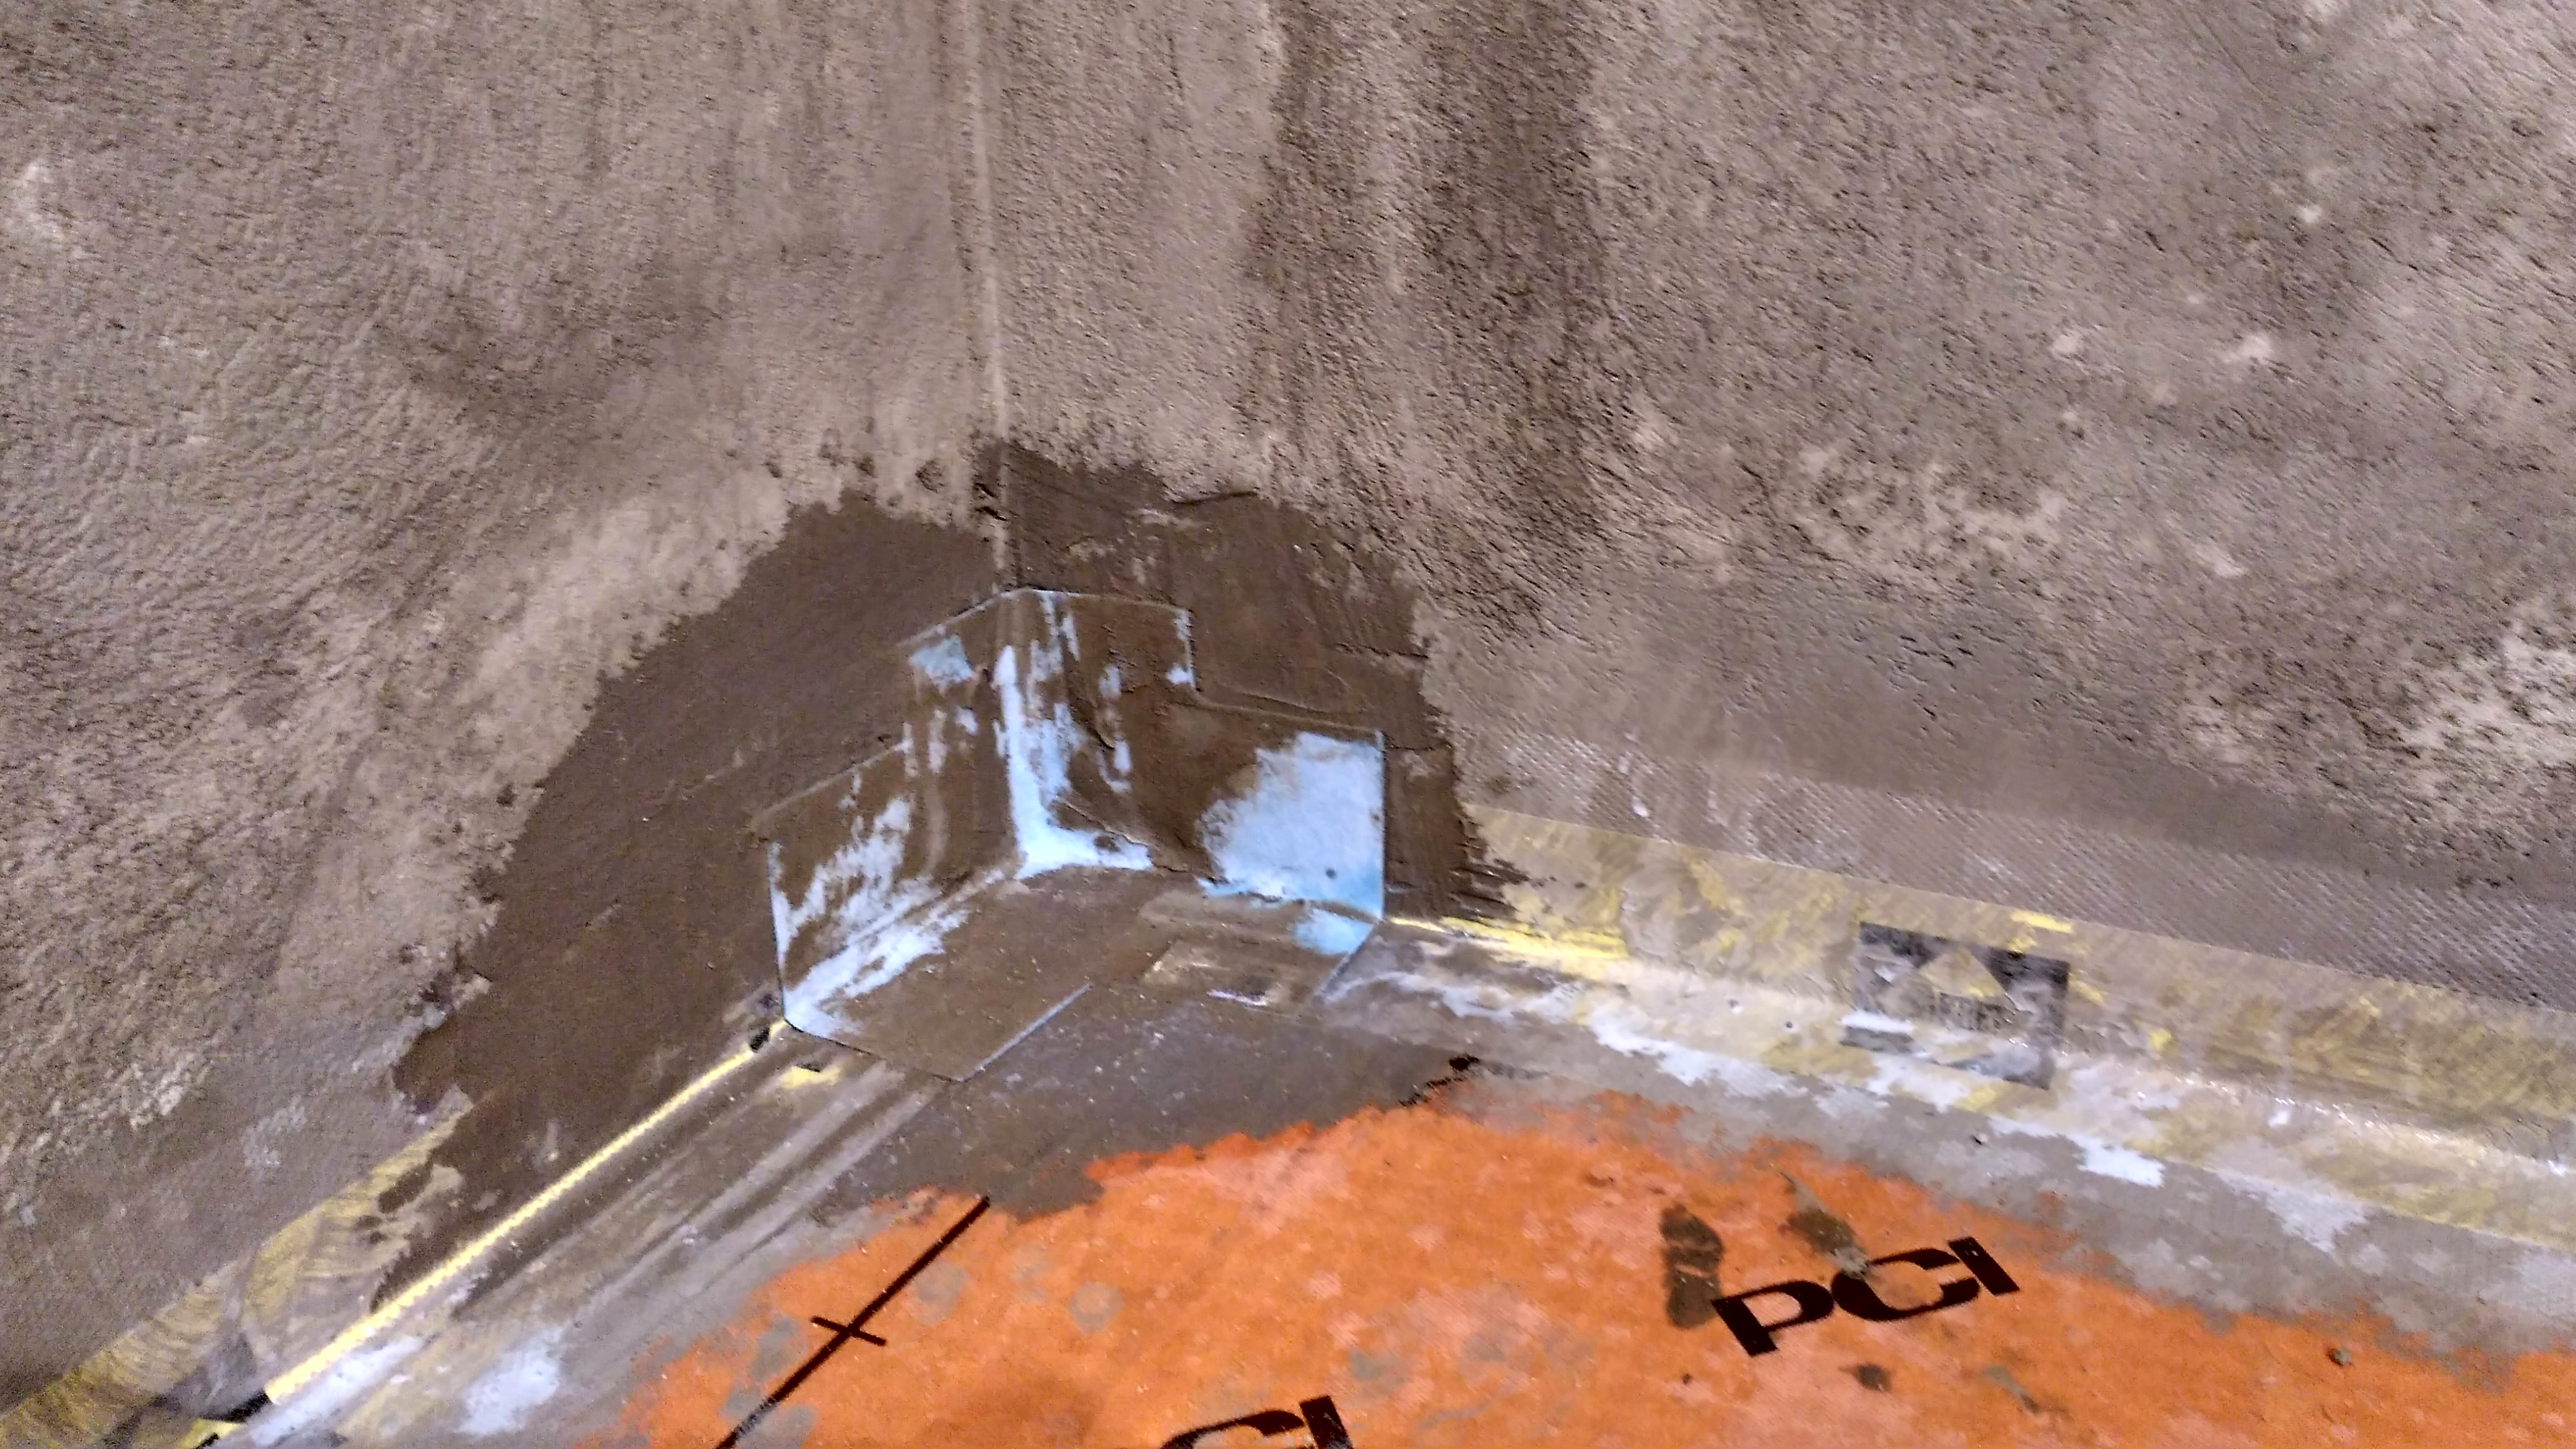
\includegraphics[scale=0.1]{Resources/Praktikum/IMG_20180801_114836_HDR.jpg}
		\label{eckeDicht}
		\caption{Ecke mit Abdichtbändern}	
	\end{center}
\end{figure}

Nun mussten die Wände der Dusche den Vorschriften gemäß wasserdicht gemacht werden. Nur Fliesen alleine bieten einen ungenügenden Schutz gegen Wasser. Dazu strich ich die gesamte Dusche mit Lastogum, einer Flüssigfolie aus. Diese bildet auf der Mauer eine Wasserundurchlässige Schicht. In den Kanten der Dusche mussten Abdichtbänder eingeklebt werden. Dazu schnitt ich nach Augenmaß die Bänder zurecht. Anschließend strich ich dick Flüssigfolie in die Kanten und klebte das Abdichtband ein (siehe Abbildung \ref{duscheDicht}). Währenddessen bestrich der Fliesenleger den Periplanboden mit Hilfe einer feinzahnigen Kelle mit Kleber und legte die Entkopplungsmatten darauf (siehe Abbildung \ref{bodenDicht}). Die Kelle mit 2mm Stärke benutzte er, damit er den Kleber nicht zu dick aufträgt, damit die Matte nicht schwimmt und wellig wird. Daraufhin klebte ich die Abdichtbänder auch in die Kanten des Bodens, auf die Entkopplungsmatten. Der Fliesenleger klebte danach noch Abdichtecken in alle Ecken des Raums, um ihn komplett wasserdicht zu machen (siehe Abbildung \ref{eckeDicht}). Anschließend grundierten wir den Boden und alle Wände. Dann war alles bereit zum Fliesenverlegen.

\subsection{Fliesen verlegen und verfugen}

Der Fliesenleger wollte zuerst die Wandfliesen verlegen. Dazu bestimmte er anfangs noch einmal ganz genau die Länge der ersten Wand. Er bestimmte zusätzlich ob der Boden entlang der Wand gerade verlief, oder ob sich Unebenheiten zeigten. Damit wollte der den Verschnitt bestimmen, den er am Boden haben wird, oder ob der, bei geradem Boden, ganze Fliesen bis nach unten verlegen konnte. Er wollte ca. auf Schulterhöhe mit dem Verlegen beginnen. Dazu zeichneten wir eine horizontale Orientierungslinie mit einer Schlagschnur an. Durch diese Linie konnte er sichergehen, dass die Wandfliesen nicht schief wurden, wenn er von einer Seite der Wand zur anderen verlegte. Er strich mit einer gezahnten Kelle Kleber, genug für zwei aneinanderliegende Fliesen, an die Wand und klebte eine Fliese ein. Beim Einkleben der zweiten Fliese ließ er für die Fuge ca. 5mm Platz zur ersten Fliese. Das machte er nach Augenmaß, ohne Abstandshalter. So klebte er eine Linie Fliesen vom einen Ende der Wand zum Anderen, entlang der Orientierungslinie ein. Bis jetzt konnte er dafür ganze Fliesen verwenden, die letzte musste er zuschneiden.

\begin{figure}[h]
	\begin{center}
		\noindent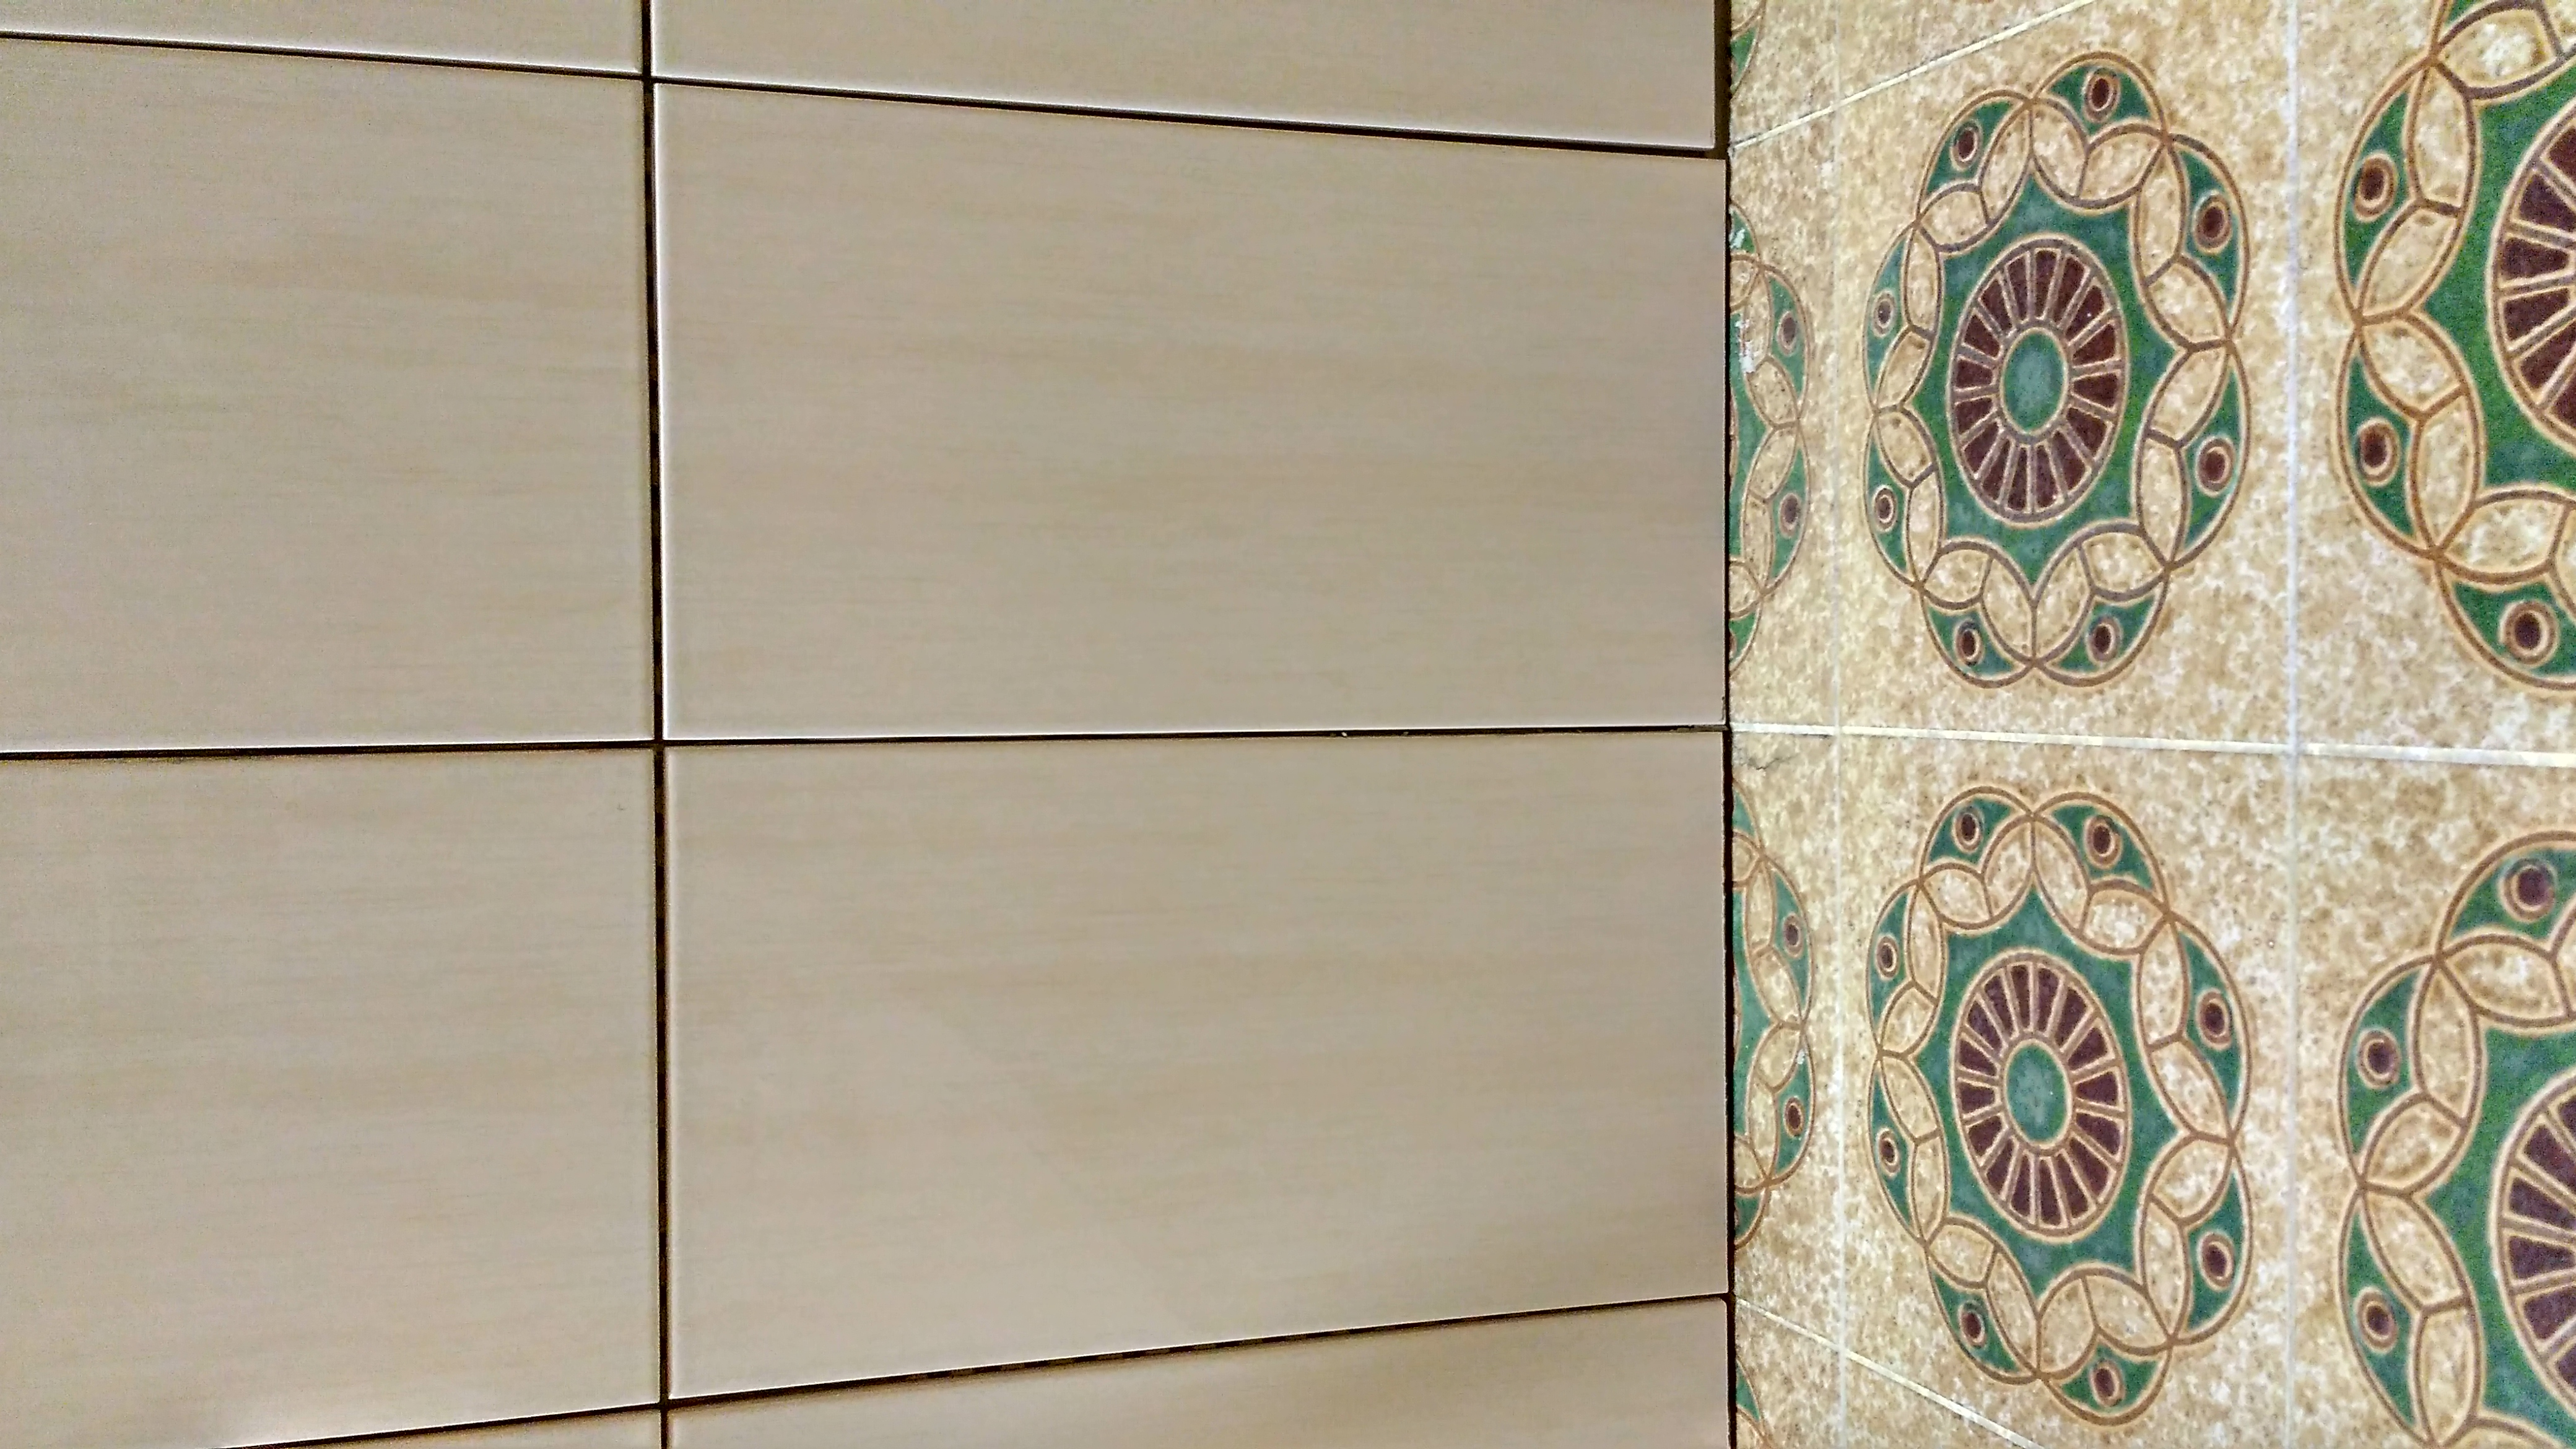
\includegraphics[scale=0.1]{Resources/Praktikum/IMG_20180806_081044_HDR.jpg}
		\label{wandFlieseSchneiden}
		\caption{Geschnittene Fliesen am Ende der ersten Wand}	
	\end{center}
\end{figure}

\begin{figure}[h]
	\begin{center}
		\noindent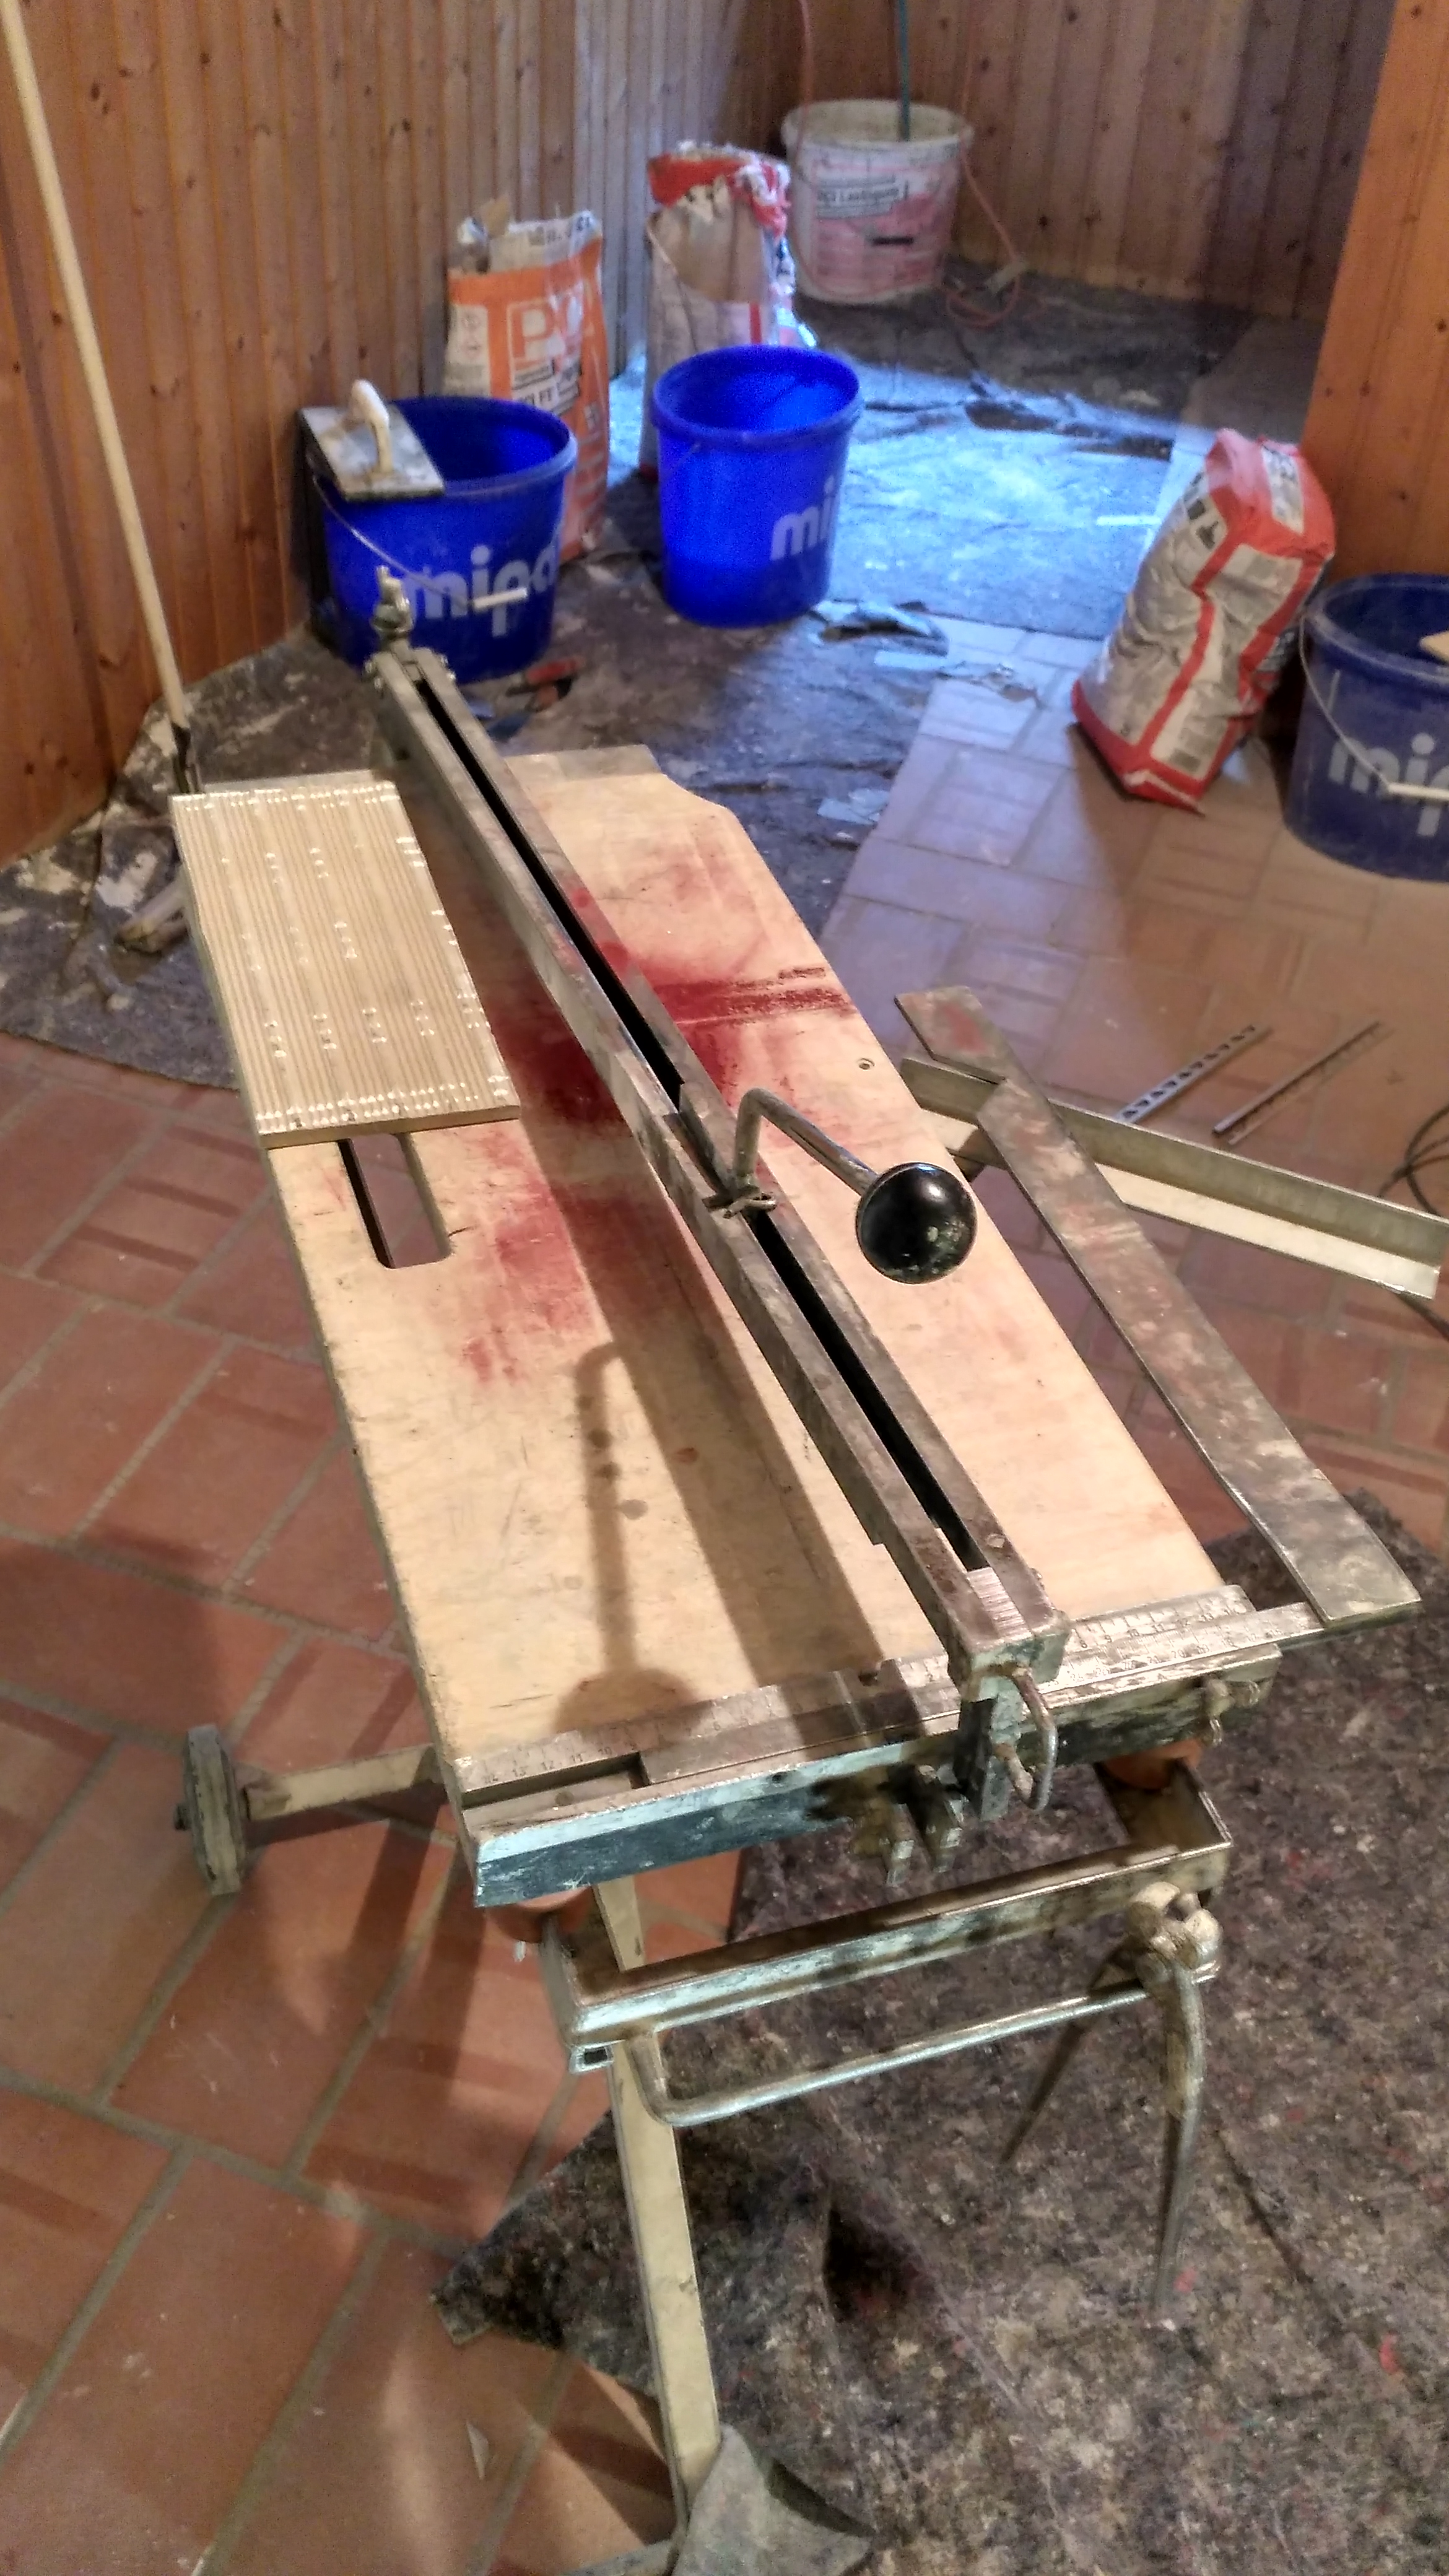
\includegraphics[scale=0.1]{Resources/Praktikum/IMG_20180807_120442_HDR.jpg}
		\label{schneider}
		\caption{Schneidebrett}	
	\end{center}
\end{figure}

Er maß den Abstand der letzten Fliese zur Wand. Auf seinem Fliesenschneider konnte er das Maß darauf einstellen, legte die Fliese ein, fuhr einmal mit dem Schneider darüber und brach das unbenötigte Stück entlang der Schnittlinie ab. Der gesamte Vorgang dauerte nicht länger als eine Minute.

Die zugeschnittene Fliese brachte er am Ende der Wand an. Anschließend klebte er die zwei Reihen darunter usw. ein (siehe Abbildung \ref{wandFlieseSchneiden}). Danach schlugen wir wieder eine horizontale Orientierungslinie an die Wand. Das machten wir regelmäßig, um zu gewährleisten, dass die Fliesenreihe nicht schief wurde. So flieste er die gesamte Wand, während ich ihm die Fliesen reichte.

\begin{figure}[h]
	\begin{center}
		\noindent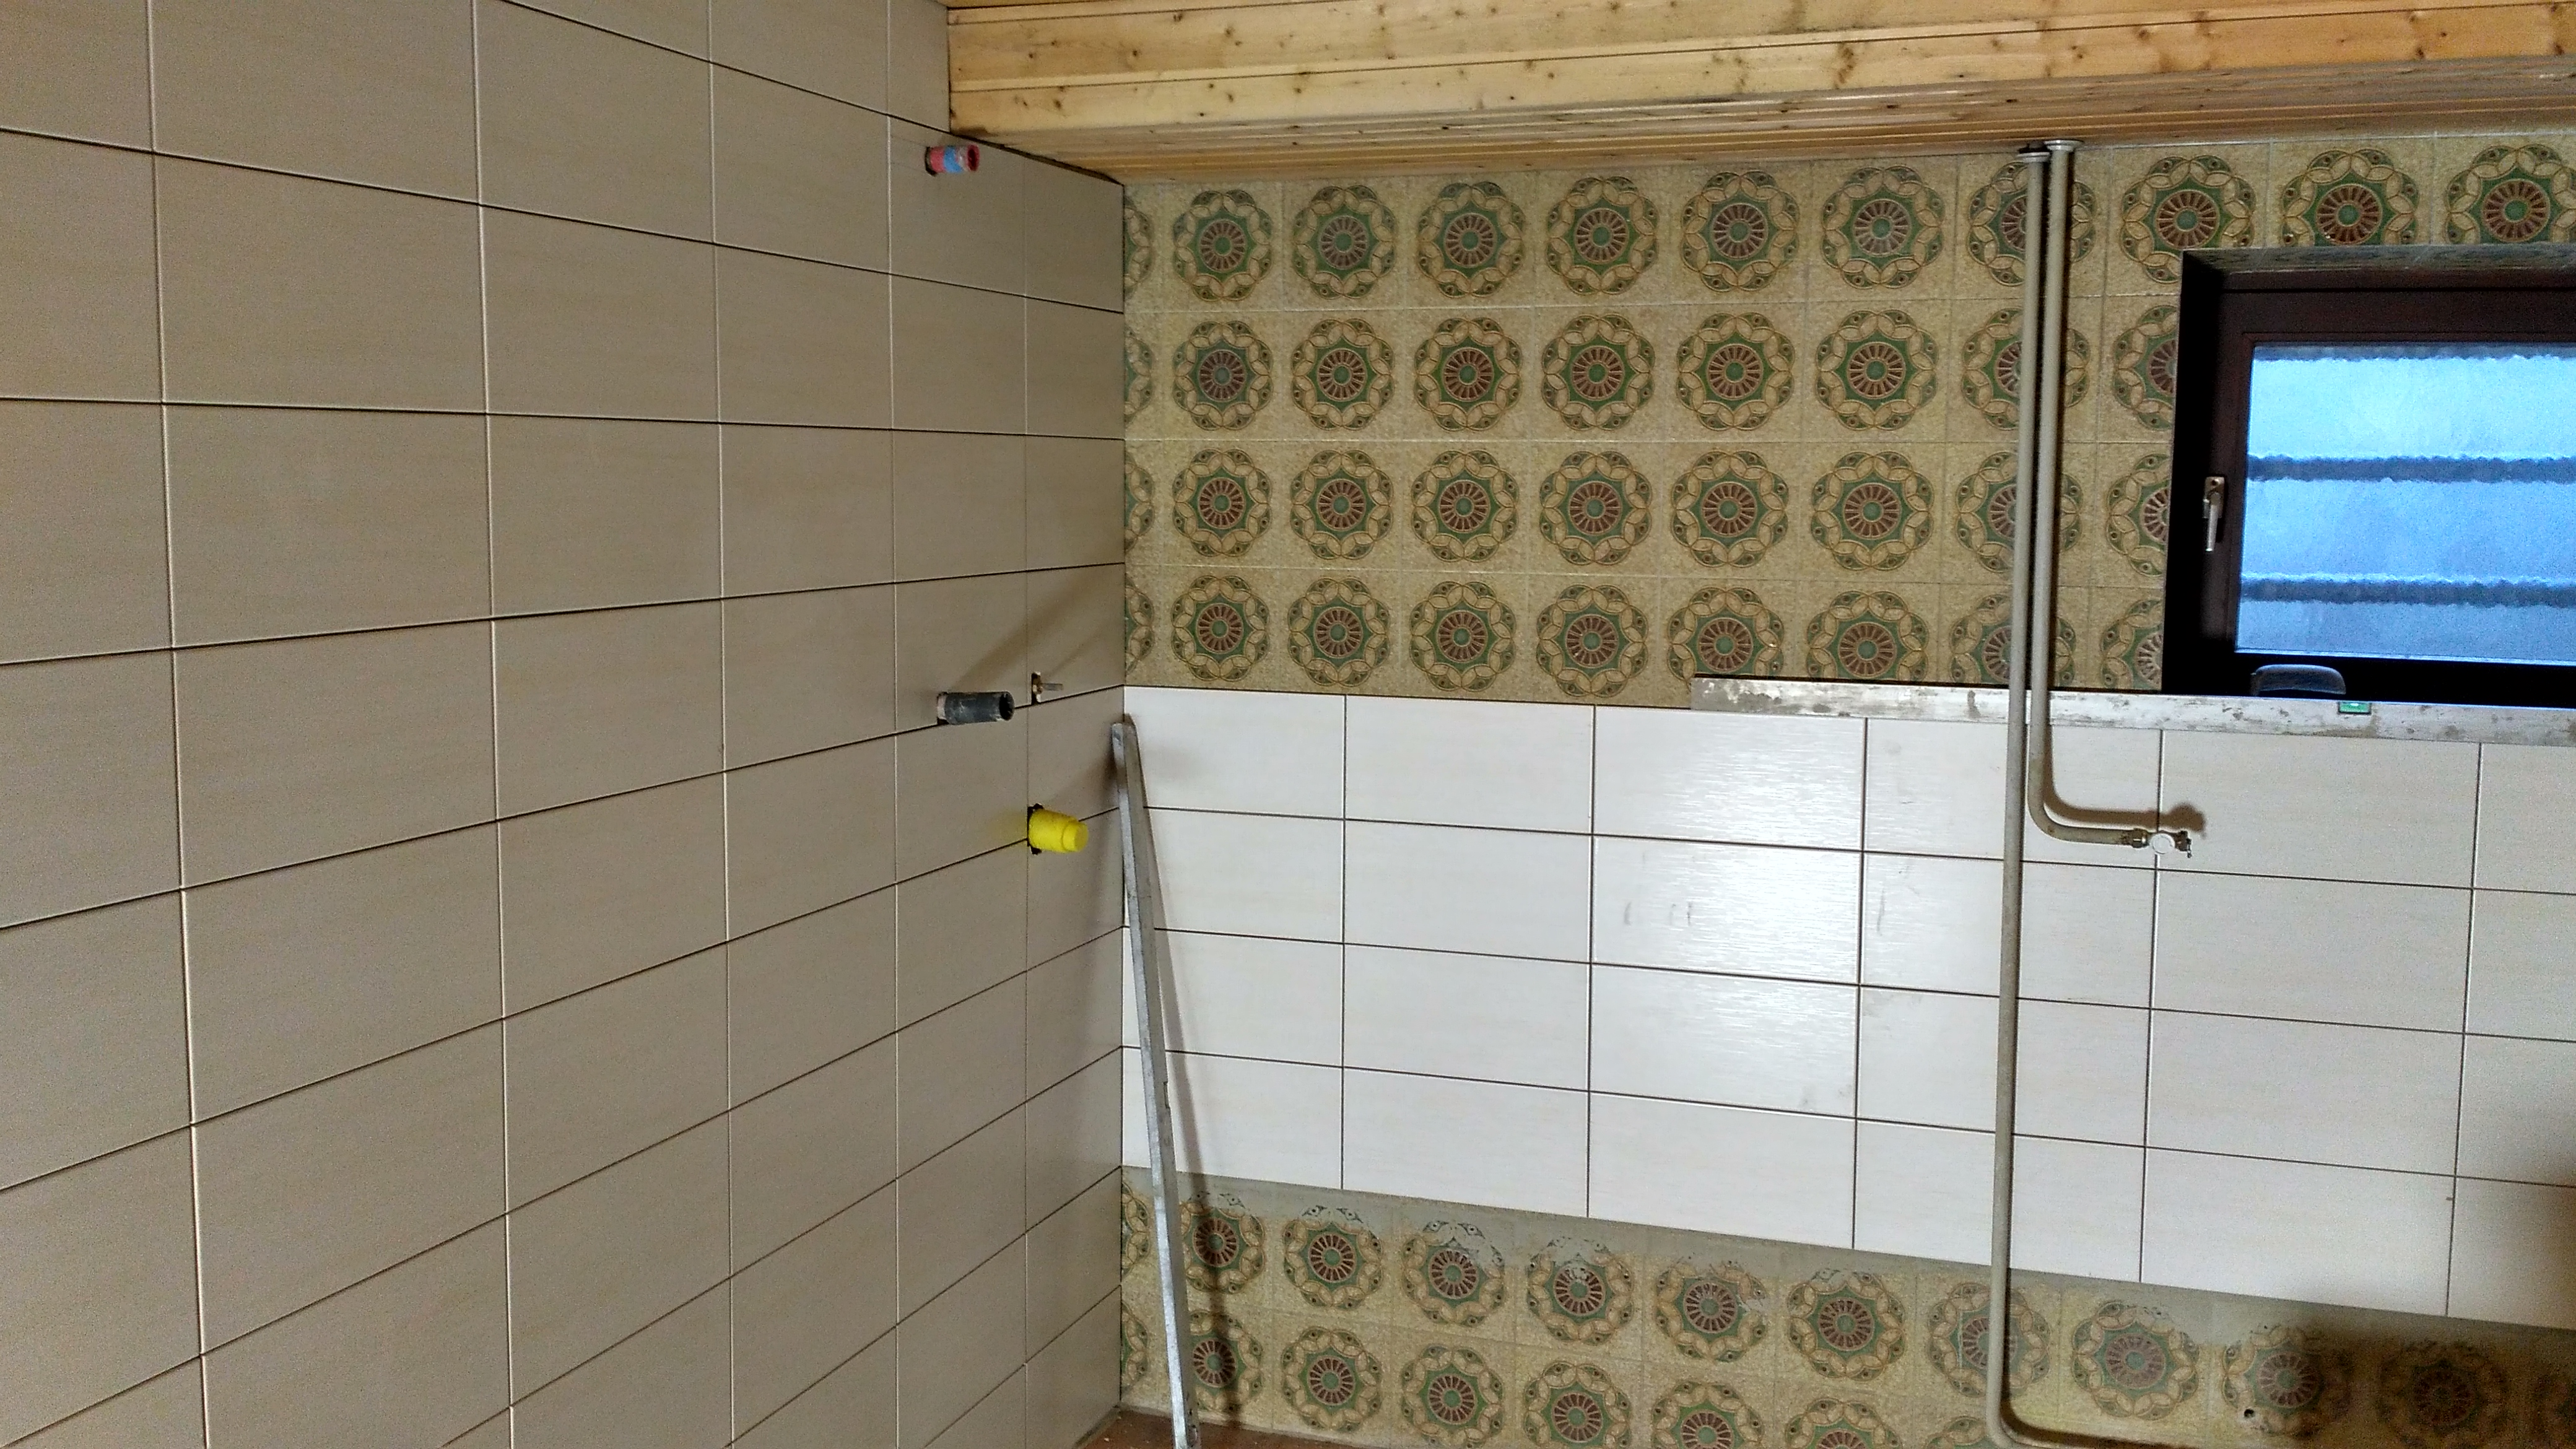
\includegraphics[scale=0.1]{Resources/Praktikum/IMG_20180806_081011_HDR.jpg}
		\label{ersteWand}
		\caption{Fertige erste Wand und Anfang der Zweiten}	
	\end{center}
\end{figure}

Sobald die erste Wand fertig verfliest war begann er mit den anderen und ich fing an die Fliesen zu verfugen. Dazu strich ich mit einer Kelle dick Fugenmasse in die Zwischenräume der Fliesen. Anschließend wischte ich mit einem feuchten Schwamm darüber, um die überschüssige Fugenmasse abzutragen und der Fuge ihr richtiges Aussehen zu geben. Zum Schuss zog ich den frisch ausgewaschenen Schwamm einmal komplett von oben nach unten über die Wand, um die Fliesen sauber zu waschen. So ging ich auch bei den anderen Wänden vor.

\begin{figure}[h]
	\begin{center}
		\noindent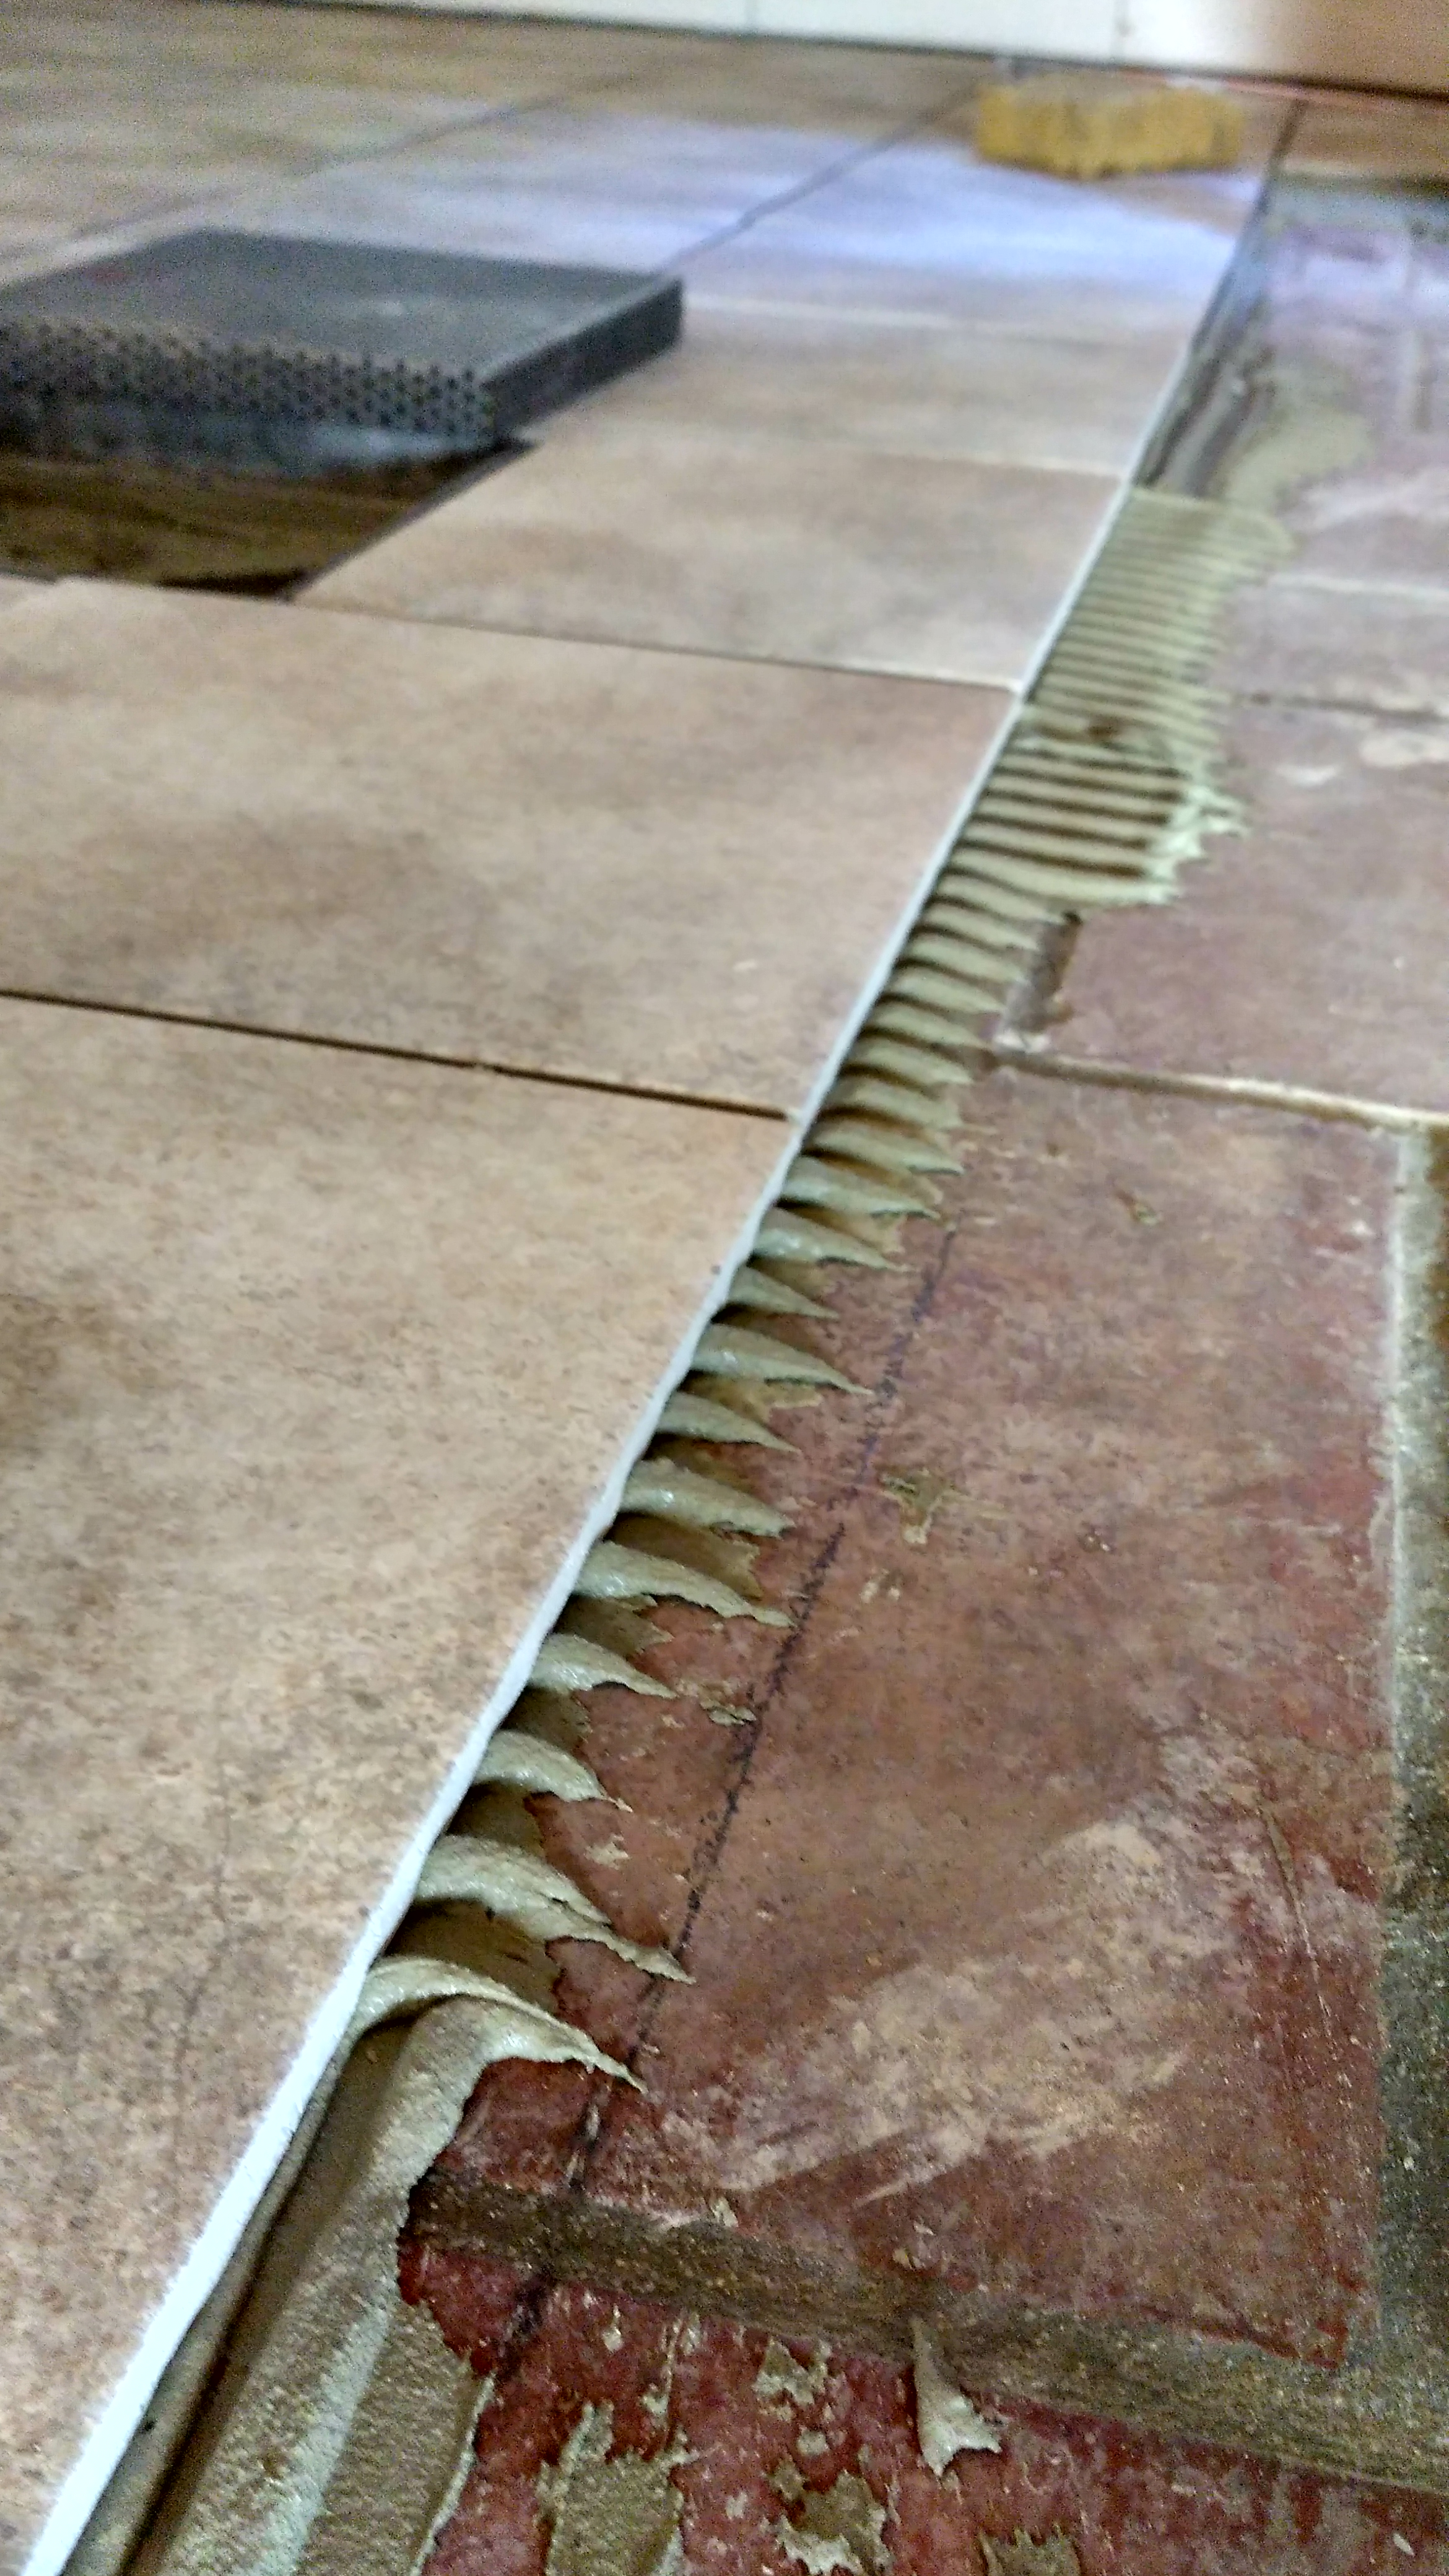
\includegraphics[scale=0.1]{Resources/Praktikum/IMG_20180807_112239_HDR.jpg}
		\label{orientierung}
		\caption{Orientierungslinie zum Verlegen der Bodenfliesen}	
	\end{center}
\end{figure}

Nach dem Verlegen der Wände begann er mit dem Boden. Durch den Periplanboden war sichergestellt, dass keine Unebenheiten vorhanden sind. Sollte die Mitte des Raumes beispielsweise einen Abfluss haben und man müsste den Boden zu diesem abfallen lassen, müsste der Fliesenleger das beim Verlegen mit einplanen. Hier hatten wir aber einen ebenen Boden. Nun zeichneten wir mit der Schlagschnur wieder eine Orientierungslinie parallel zur Wand ein, ca. so weit von dieser entfernt, wie die Breite zweier aneinandergelegter Fliesen (siehe Abbildung \ref{orientierung}). Ich platzierte einige Bodenfliesen so, dass der Fliesenleger direkt darauf zugreifen kann, während er am Boden kniet und die Fliesen verlegt. Er strich den Kleber auf den Boden und verteilte ihn mit einer gezahnten Kelle. Danach legte er die Fliesen darauf. Den Abstand zweier Fliesen für die Fuge bestimmte er per Augenmaß. Die Orientierungslinie diente dazu, dass die Fliesen nicht schief wurden, da er alles nach Augenmaß verlegte. 

Nachdem er zwei Reihen Fliesen verlegt hatte, stand er auf und wir zeichneten eine weitere Orientierungslinie, zwei Fliesenbreiten weiter, ein. Dann wiederholte sich der ganze Prozess, bis der Boden komplett verlegt war. Mir viel dabei auf, dass der Arbeitsfluss des Fliesenlegers durch das anzeichnen der Orientierungslinie immer wieder unterbrochen wurde. 

Zum Schluss, nachdem der Kleber eine Nacht ausgehärtet hatte, verfugte ich die Bodenfliesen noch. Dazu strich ich, wie beim Verfugen der Wandfliesen, Fugenmasse zwischen die Fliesen, wischte mit feuchten Schwamm darüber, bis sie das ge-wünschte Aussehen hatten und wusch die Fliesen anschließend mit dem Schwamm sauber. Nun war der gesamte Raum gefliest.

\subsection{Finale Schritte}

Nach dem Fliesen und Verfugen müssen noch ein paar kleine Schritte durchgeführt werden, um die Arbeit fertigzustellen. Wurden beispielsweise große, schwere Wand-fliesen verlegt, wurden Abstandshalter zwischen zwei Fliesen geklemmt, damit diese nicht zusammenrutschen und die Fuge so zerstören. Diese Abstandshalter müssen jetzt entfernt werden, und die Löcher in der Fuge geschlossen.

Die Fliesen wurden verlegt, bevor der Türstock eingebaut wurde. Nachdem dieser eingesetzt wurde, mussten die Zwischenräume zwischen Türstock und Fliesen verfugt werden. Dazu spritzte der Fliesenleger Acrylsilikon hinein und strich es mit einem Schaber glatt. Acrylsilikon hat die Eigenschaft, Farbe, mit welcher er überstrichen wird, aufzunehmen und so besser zu halten.

\subsection{Besorgungsfahrten}
Um den Lesefluss nicht zu unterbrechen, habe ich Besorgungsfahrten in den Baumarkt oder Fahrten in das Lager nicht aufgenommen. Hier möchte diese zwei Aspekte kurz beschreiben.

Der Fliesenleger hat ein privates Lager, in dem er nicht verbrauchte Materialien, seine Utensilien, wie Kellen und Eimer, und Werkzeuge, wie ein Multitool aufbewahrt. Den Lagerbestand hat er im Kopf. Am Anfang jedes Tages fuhren wir zuerst in das Lager und packten die nötigen Sachen ein. Da sein Auto nicht zu groß war, war die Tagesplanung wichtig, um unnötige Lagerfahrten während des Tages zu vermeiden.

Hatte er etwas nicht im Lager, was wir für die Baustelle brauchten, kauften wir es im Baumarkt ein. Alle Handwerker sind gut mit Baumärkten vernetzt. Sie können anrufen und vorbestellen. Die Baumärkte bereiten die Materialien dann vor, sodass man sie schnell abholen kann. Noch dazu speichern die Märkte die Daten des Handwerkers und können so direkt Abrechnungen erstellen und ihm zukommen lassen. Das spart wiederum Zeit, da man nicht zum Bezahlen in der Schlange stehen muss.

\section{Herausgearbeitete Ansatzpunkte}

Durch die Ethnographie zeigt sich, dass die meisten Arbeitsschritte eines Fliesenlegers relativ schnell auch präzise ausgeführt werden können. Kleber und sonstige Stoffe anzumischen erfordert keine Hilfe. Wände mit Flüssigkleber, Boden oder Wände mit Fliesenkleber und Fugen mit Fugenmasse zu bestreichen, lässt sich mit geeignetem Werkzeug präzise und schnell ausführen. Auch für das Schneiden und Einkleben der Fliesen sind die Maße schnell genommen und eingezeichnet. Der Fliesenleger hat eine einstudierte Routine und arbeitet dadurch zügig.
Allerdings werden zwei Ansatzpunkte deutlich, bei denen der Handwerker Unterstützung benötigt. Das sind die Planung mit dem Kunden im Kundengespräch, wobei Kunde und Fliesenleger gerne aneinander Vorbeireden, oder der Kunde sich das Ergebnis nicht vorstellen kann, sowie das Fliesenlegen, wo der Fliesenleger durch das anschlagen der Orientierungslinie aus dem Arbeitsfluss gerissen wird.

\subsection{Unterstützung beim Fliesenlegen}

Wenn der Fliesenleger ohne Orientierungslinie arbeitet, läuft er Gefahr, den Boden irgendwann schief zu verlegen. Ohne sie kann er also nicht arbeiten. Jedes mal wenn er diese mit der Schlagschnur anzeichnet, muss er aufstehen, die Endpunkte der Linie markieren und diese einzeichnen. Das wird nochmal schwerer, wenn er allein arbeitet, da man eine Schlagschnur mit zwei Personen leichter benutzen kann. Das anzeichnen reißt ihn zusätzlich aus seinem Arbeitsfluss. Könnte der Fliesenleger den Schritt des Anzeichnens einer Orientierungslinie umgehen, könnte er ungehindert weiterarbeiten, sofern er einen Helfer hat der ihm die Fliesen reicht und Kleber für ihn anrührt. Dadurch kann er viel Zeit sparen und es wäre gleichzeitig auch bequemer für ihn.

\subsection{Unterstützung beim Kundengespräch}

Das Kundengespräch war chaotisch und sehr unstrukturiert. Die Vorstellungskraft der Kunden, vor allem wenn diese Laien sind, ist sehr begrenzt. Dadurch ist es schwer mit ihnen über Änderungen zu diskutieren. Der Fliesenleger hat das Bild, durch seine Erfahrung besser im Kopf. Jedoch ist es schwer das in Worte zu fassen die der Kunde versteht. Es wäre deutlich einfacher über Ideen zu sprechen, wenn man diese direkt vor sich sehen würde.

Das Ergebnis vorab schon zu sehen hat noch weiter Vorteile:

\begin{itemize}
	\item Der Kunde kann während dem Planungsprozess bereits gezielt Feedback geben. Ansonsten kann er das erst spät im Prozess, wodurch es erheblich schwerer ist darauf einzugehen.
	\item Dadurch kann der Vertrag mit dem Kunden, was der Fliesenleger zu tun hat, genauer ausgearbeitet werden.
	\item Die Zusammenarbeit mit anderen Handwerkern ist einfacher koordinierbar.
	\item Das geplante Muster dient als visuelle Vorlage für den Fliesenleger. Dadurch muss er das Bild nicht nur im Kopf haben.
	\item Bereits beim Planen des Raumes lässt sich der Verschnitt gut abschätzen.
\end{itemize}

Die Unterstützung bei der Orientierungslinie würde dem Fliesenleger Zeit ersparen und ein Visualisierungstool würde ihm die Planung erleichtern. Daran kann man ansetzen, um technische Unterstützungssysteme zu implementieren.